\documentclass[lang=cn,newtx,11pt,scheme=chinese]{elegantbook}
\usepackage{physics}
\usepackage{simpler-wick}
\usepackage{tikz-feynman}



\usepackage{fancyhdr}
\pagestyle{fancy}
\fancyhead[L]{
    \begin{minipage}[c]{0.06\textwidth}
        \centering
        \includegraphics[height=7.5mm]{院徽.jpg}
    \end{minipage}
    \begin{minipage}[c]{0.4\textwidth}
    The Note of Quantum Field Theory
    \end{minipage}
}
\fancyfoot[C]{\thepage}


\title{Note of Quantum Field Theory}
\author{Kaiser\\University of South China}




\setcounter{tocdepth}{3}

\logo{院徽.jpg}
\cover{cover.png}

% 本文档命令
\usepackage{array}
\newcommand{\ccr}[1]{\makecell{{\color{#1}\rule{1cm}{1cm}}}}

% 修改标题页的橙色带
\definecolor{customcolor}{RGB}{32,178,170}
\colorlet{coverlinecolor}{customcolor}
\usepackage{cprotect}



\begin{document}

\maketitle

\thispagestyle{plain} 

\frontmatter


\tableofcontents


\nocite{*}
\bibliographystyle{plain}
\bibliography{refs}


    % \begin{thebibliography}{99} 
    %     \bibitem{1} David Tong,\textit{Quantum Field Theory}
    %     \bibitem{2} M.Peskin and D.Schroeder,\textit{An Introduction of Quantum Field Theory}
    %     \bibitem{3} A.Zee,\textit{Quantum Field Theory in a Nutshell}
    %     \bibitem{4} S.Weinberg,\textit{The Quantum Theory of Field (Volume 1)}
    %     \bibitem{5} Landau,Lev D.,and Lifshitz,E.M.,\textit{The Classical Theory of Field}
    %     \bibitem{6} 高显,\textit{经典力学}
    %     \bibitem{7} 陈童,\textit{经典场论}
    %     \bibitem{8} 埃格先生,\textit{微分流形与分析力学初步}
    %     \bibitem{9} 陈童,\textit{经典力学新讲}
    %     \bibitem{10} Tom Lancaster,Stephen J.Blundell,\textit{Quantum Field Theory For Gifted Amature}
    % \end{thebibliography}






\mainmatter
\newpage





\chapter{\protect\hyperlink{:}{经典力学、经典场论与狭义相对论复习}}
\addtocontents{toc}{\protect\hypertarget{:}{}}
有一定的量子场论基础的人都知道,即使没有经典场论的基础(或者说是没有经典连续场的基础)也是无伤大雅的,因为量子场可以不依赖于经典连续场引入,但是就我个人认为,学习和重温量子场论中的基本概念以及很多的处理方法是必要的。同时,从经典场出发进行量子化得到粗糙的量子场,再根据其存在的漏洞进行正规化、重整化以获得具有预言能力的量子场论。

在这一部分,或者说这一次汇报中,我将讨论经典力学,经典场论以及狭义相对论的几个方面。


\section{\protect\hyperlink{:}{伽利略变换}}
\addtocontents{toc}{\protect\hypertarget{:}{}}
考虑两个沿着$x$轴方向相对运动的惯性观察者,在$t=0$时,两者是互相重合的,并且我们假设它们之间的相对运动的速度(即相对速度)为常数,他们将会分别对应到两个参考系$S$和$S^\prime$,我们可以给出它们此时之间的坐标变换关系:
\begin{align*}
    S\to S^\prime:
    \begin{cases}
        &t^\prime=t\\
        &x^\prime=x-vt\\
        &y^\prime=y\\
        &z^\prime=z
    \end{cases}
\end{align*}

我们将其使用矩阵语言来进行表示就是:
\begin{align*}
    \begin{pmatrix}
        t^\prime\\x^\prime\\y^\prime\\z^\prime
    \end{pmatrix}
    =
    \begin{pmatrix}
        1&0&0&0\\
        -v&1&0&0\\
        0&0&1&0\\
        0&0&0&1
    \end{pmatrix}
    \begin{pmatrix}
        t\\x\\y\\z
    \end{pmatrix}
\end{align*}

同时,值得注意的是,我们连续地做两次伽利略变换得到的还会是伽利略变换,对于任意一个伽利略变换也都存在一个逆变换(将速度从$v$改成$-v$即可),当$v=0$时的伽利略变换将会是一个恒等变换,当然,伽利略变换也满足结合律,这也就是说,伽利略变换在数学上是构成了一个群的,并且,由于该群的变换参数$v$是一个可以连续变化的,因此他将对应着一个连续群(李群)的数学结构,叫作“伽利略变换群”,并且,容易发现,经典力学中的牛顿运动定律
\begin{align*}
    \vec{F}=m\vec{a}=m\frac{d^2}{dt^2}\vec{x}
\end{align*}

在伽利略变换下可以保持数学形式不变,用现代理论物理的语言来说,这意味着伽利略变换时牛顿运动定律的一个对称性,但是,其所导出的速度的相对关系为
\begin{align*}
    u^\prime&=\frac{d x^\prime}{dt^\prime}\\
    &=\frac{d(x-vt)}{dt}\\
    &=u-v
\end{align*}

很显然,这是非常符合日常生活经验和直觉的,直到迈克尔逊莫雷实验的出现,告诉我们,\textbf{真空中光速不变},但是很显然,伽利略




\section{\protect\hyperlink{:}{经典力学}}
\addtocontents{toc}{\protect\hypertarget{:}{}}
写这一部分的内容,主要是为了让接下来在讲解经典力学以及经典场论时都有一定的物理基础,并且明白,为什么我们的拉格朗日力学所研究的空间是位形空间,需要的是广义坐标$q$,广义速度$\dot{q}$,而哈密顿力学研究的是相空间,使用的是正则坐标$q$,正则动量$p$。在搞明白了这些之后,我们才能真正的理解经典力学,并且向着经典场论靠近。


\subsection{\protect\hyperlink{:}{位形、位形空间、广义坐标、广义速度}}
\addtocontents{toc}{\protect\hypertarget{:}{}}

\subsubsection{\protect\hyperlink{:}{位形、位形空间}}
\addtocontents{toc}{\protect\hypertarget{:}{}}

位形,是我们对粒子在空间中的位置概念的推广,其定义我们一般写为
\begin{definition}[位形]
    粒子系统中各个粒子的空间位置,或者更一般的物流系统在空间中的形状、分布。
\end{definition}

位形既然是粒子的空间位置,因此一个物理系统的某个量与位置相关,就可以用位形描述。例如:空间中某点的粒子密度 $\rho(x)$ ,即为密度位形,某点的温度 $T(x)$ ,即为温度位形。

\begin{definition}[位形空间]
    系统所有可能的位形的集合。位形空间的一点(或者说是一个元素)即为系统可能的一种位形。
\end{definition}

位形是粒子的空间位置,位形空间是位形的集合,所以位形空间就是粒子在空间所有可能的位置的集合,例如粒子在一张二维水平面上,则粒子的位形空间就是这个水平面。粒子被限制在某个圆环内,则其位形空间就是这个圆环。

由于有时间维度的影响,物理系统会随着时间演化,从位形空间的一点转移到另外一点,其画出的曲线即为位形空间中的轨迹。但是此时,我们只是考虑了粒子位置的连续改变。如果考虑时间维度,我们可以得到如下更大的空间
\begin{figure}[hbpt]
    \centering
    \includegraphics[width = 0.5\textwidth]{figure/位形空间.png}
    \caption{位形空间随时间变化图}
\end{figure}

这条在时间维度与位形空间共同组成的空间画出的轨迹被称为世界线(world line)。

它与位形空间中的轨迹的区别在于,虽然位形空间中的轨迹与时间线都依赖于时间的演化,但是位形空间中两点 $a(t_1,x_1)$ 和 $b(t_1,x_2)$ 的连接得到的轨迹只是位形的连续变化,其轨迹上的每一点都是位形。而世界线上的任意两点的连接是在时间上的连续变化,其上的每一点都是时间。

\subsubsection{\protect\hyperlink{:}{广义坐标}}
\addtocontents{toc}{\protect\hypertarget{:}{}}

\begin{definition}[广义坐标]
    任何一组可以唯一确定系统某一位形的独立参数
\end{definition}



我们知道,对于一个空间,我们可以使用像爱因斯坦那样的,将所有的都几何化,这样我们所得到的任何的结论都将与参考系(进而是坐标系)的选取无关了,但是当我们要开始计算一些具体的东西的时候,比如某人跑了多快等问题,我们将要落实到具体的计算上,因此,我们便需要坐标并依靠坐标建立起一个度量系统来帮助我们对物理世界进行一个描述,也就是利用坐标来对空间参数化,只要给出一组数,就可以确定空间中的一点。而这组数字就被称为“坐标”。例如,对于三维空间的点粒子,我们分别有:直角坐标 $(x,y,z)$,柱坐标 $(r,\phi,z)$ ,球坐标 $(r,\theta,\phi)$
点粒子在空间中的位置的参数化是普通坐标,而位形是点粒子位置概念的推广。自然而然,我们就称对位形空间的参数化为广义坐标。

这也就告诉了我们,描述一个物理系统的广义坐标的数量应该是等于位形空间的维数的。
\begin{equation}
    \text{位形空间的维数} = \text{独立广义坐标的个数}
\end{equation}


我们知道,广义坐标是对位形空间的参数化,对于同一个物理系统,我们可以选取不同参数化的方法。一般而言,如果在一组广义坐标下复杂的运动方程,换成另一组广义坐标经常就变得容易求解。例如球对称引力场中粒子的运动,运动方程在球坐标下就比直角坐标下要简单得多。

现在假设我们有两组广义坐标 $\{q^a\} , \{\tilde{q}^a\}$ 用来描述同一个位形空间,那么对于某一个点 $P$ ,其对应的 $\{q^a\}$ 坐标的数值表示为 $ \left. q^a \right|_P$,其对应的 $\{\tilde{q}^a\}$ 坐标的数值表示为 $ \left. \tilde{q}^a \right|_P$,并且这两组坐标的数值满足函数关系
\begin{equation}
    \left.\tilde{q}^q\right|_P = f^a\left(\mathbf{q}|_P \right)
\end{equation}


\subsubsection{\protect\hyperlink{:}{广义速度、速度相空间}}
\addtocontents{toc}{\protect\hypertarget{:}{}}

我们的经典力学,在一开始被创造出来的目的就是为了研究物理系统随着时间的演化,但是如果我们想要完完全全地将一个物理系统给描述清楚,我们到底需要多少的信息呢?这一点,泰勒展开给出了答案:
\begin{equation}
    f(t) = f(t_0) + f^{\prime}(t_0)(t - t_0) + \frac{1}{2}f^{\prime\prime}(t_0)(t - t_0)^2 + \frac{1}{3!}f^{\prime\prime\prime}(t_0)(t - t_0)^3 + \cdots
\end{equation}

这告诉我们,要是想完全决定一个函数的形式,我们需要知道该函数在某一点的无限阶导数,在我们这里,就是在说,要是想完全确定一个系统的演化,我们至少要知道位置、速度、加速度、加加速度等无穷多的信息,而实际上,我们一般只需要知道一个系统的位置与速度即可,这也就是说,我们至少要有如下的关系
\begin{equation}
    f^{\prime\prime}(t) = F(f(t),f^{\prime}(t))
\end{equation}
基于此关系,我们会发现,三阶导数可以被表达为
\begin{equation}
    f^{\prime\prime\prime}(t) = \frac{d}{dt}F(f(t),f^{\prime}(t)) = \frac{\partial F}{\partial f} f^\prime + \frac{\partial F}{\partial f^\prime} f^{\prime\prime} = \frac{\partial F}{\partial f} f^\prime + \frac{\partial F}{\partial f^\prime}F(f,f^{\prime})
\end{equation}
即,我们的三阶导数也能够被函数和一阶导所决定,对于更为高阶的导数,也可以不断地往下类推,于是我们要想描述出一个物理系统,知道位置和速度就足够了。

所以,只要系统的位形的演化能够满足一个二阶微分方程,那么知道此时此刻的广义坐标($q$)以及广义速度($\dot{q}$)就可以完完全全地确定此后任意时刻系统的演化。既然广义速度与广义坐标可以包含系统演化的全部信息,我们便可以将广义速度与广义坐标合在一起组成一个能够确定系统的物理状态的态(state),而对于这些所有状态的合集,即为状态空间,称为 $\textbf{相空间}$,而我们的相空间的维数即为
\begin{equation}
    \text{相空间的维数} = \text{唯一确定系统演化的独立参数的个数} 
\end{equation}
对于点粒子系统,我们的速度相空间(就是由广义坐标与广义速度张成的相空间)总是偶数维的。

将时间轴加入进来,速度相空间中的点也随时间演化扫出一条条的曲线来,如图\ref{fig:velocity-phase-space}所示。但是因为给定一个时刻的状态,就唯一决定了此前和此后所有时刻的状态。所以速度相空间中的点随时间扫出的曲线是永不相交的。
\begin{figure}[hbpt]
    \centering
    \includegraphics[width = 0.5\textwidth]{figure/速度相空间.png}
    \caption{速度相空间随时间变化图}
    \label{fig:velocity-phase-space}
\end{figure}

\subsubsection{\protect\hyperlink{:}{约束、自由度}}
\addtocontents{toc}{\protect\hypertarget{:}{}}
\begin{definition}[约束]
    在物理系统的状态空间中,约束是指由于运动学上的限制,系统的广义坐标与广义速度仅能取值于状态空间的某个子空间,从而导致部分状态不可达的条件。这些限制规定了系统可实现的运动范围和可能的演化路径。
\end{definition}

这个定义耶告诉了我们,约束是“运动学”的概念,与相互作用、动力学无关。

事实上,对于约束,有很多的分类方式,例如:对是否显含时间来分,则分为定常约束和非定常约束;根据约束方程是等式还是不等式来分,则分为双侧约束和单侧约束。但是我们最为常用的分类,则是完整约束(几何约束)和非完整约束。

对于完整约束,其为广义坐标之间的约束关系,通过这样的约束,我们可以知道有一些广义坐标其实并不是独立的,我们完全可以将其用别的广义坐标来表示。如果一个系统的所有约束都是完整约束,那么我们称这样的系统为\textbf{完整约束系统(holonomic\ system)}。

接下来,设一个系统,用 $m$ 个位形参量 ${q^1,\cdots,q^m}$ 描述的系统,存在且仅存在 $k$ 个独立的完整约束
\begin{equation}\label{eq:yueshu}
    \phi_\alpha (t_,q^1,\cdots,q^m) = 0,\qquad \alpha = 1,2,\cdots,k
\end{equation}
则系统的广义坐标数为
\begin{equation}
    s = m - k
\end{equation}

这就表明,如果一个系统由 $N$ 个粒子组成,并且存在 $k$ 个完整约束,如果我们使用牛顿力学的话,我们需要求解 $N$ 个运动方程,以及 $k$ 个约束方程,即 $(3N + k)$ 个方程(并且极大可能是互相耦合的),这将会使得系统的求解变得非常困难,而拉格朗日力学,如果我们一开始就选择出合适的广义坐标 ${q^1,q^2,\cdots,q^{3N - k}}$ ,那么我们将只需要求解这 $(3N - k)$ 个独立的广义坐标方程,这将会极大地降低我们求解该系统的难度。

但是我们还有另外一种约束,非完整约束(non-holonomic\ system),即不可以写为式 $\ref{eq:yueshu}$形式的约束,其中最为典型以及重要的便是\textbf{不可积微分约束(non-integrable\ differential\ constraints)}其为广义坐标与广义速度之间的约束关系,这种约束关系不能通过积分得到广义坐标的关系,因此我们不能将其用其他的广义坐标来表示,比如这个样子:
\begin{equation}
    \phi(t,q^1,\cdots,q^m,\dot{q}^1,\cdots,\dot{q}^m) = 0
\end{equation}


但是也存在一些可积的微分约束,对于这类微分约束也是完整约束。

对于存在非完整约束的一个系统,我们都将其称之为\textbf{非完整约束系统(non-holonomic\ system)}。

事实上,完整约束直接消除了广义坐标之间的独立性,表明广义坐标之间有约束关系。
这种关系既体现在广义坐标之间,也体现在广义坐标的“变分”之间。由约束方程 $\phi(t,\vec{q})$ 变分可以得到
\begin{equation}\label{eq:constraint-variation}
    \delta \phi = \sum_{a = 1}^{m} \frac{\partial \phi}{\partial q^a} \delta q^a = 0
\end{equation}

这表明广义坐标的变分之间也并非是独立的,而是满足如式 $\ref{eq:constraint-variation}$ 的线性关系的,并且有很直观的几何意义,如图 $\ref{fig:constraint-variation}$

\begin{figure}[hbpt]
    \centering
    \includegraphics[width = 0.5\textwidth]{figure/constraint-variation.png}
    \caption{完整约束变分的几何意义}
    \label{fig:constraint-variation}
\end{figure}

一个完整约束可视为位形空间中的一张曲面,系统的位形限制在这张曲面上,因此广义坐标的变分也必然限制在约束面上,而式 $\ref{eq:constraint-variation}$ 中的 $\displaystyle \frac{\partial \phi}{\partial q^a}$ 即为约束面在位形空间的梯度,也即约束面的法向量 $\nabla \phi$,同时式 $\ref{eq:constraint-variation}$ 也表明广义坐标变分 $\delta \vec{q}$ 与约束面的法向量 $\nabla \phi$ 垂直,即切于约束面。

对于非完整系统无法用代数方法消除广义坐标之间的独立性,但是因为广义速度之间存在约束关系,这就同样导致广义坐标的“变分”之间存在关系。

综上所述,对于完整系统,每一个完整约束都可以降低一个独立广义坐标变分的数目;对于非完整系统,其中的非完整约束,虽然不能够降低独立广义坐标的数目,但是能够降低独立广义坐标“变分”的数目,这也表明相较于广义坐标的数目本身,广义坐标变分的数目更加能够反映出系统的性质,这也是我们定义自由度的时候并没有将其定义为独立广义坐标数目而是定义为独立广义坐标变分的数目的原因。

\begin{definition}[自由度]
    独立广义坐标变分的数目
\end{definition}

同时,我们还有如下的关系:
\begin{equation}
    \text{自由度} = \frac{1}{2} \times \text{相空间的维数}
\end{equation}





\subsection{\protect\hyperlink{:}{相对论时空}}
\addtocontents{toc}{\protect\hypertarget{:}{}}

\subsubsection{\protect\hyperlink{:}{时空}}
\addtocontents{toc}{\protect\hypertarget{:}{}}
在物理学当中,事件(event)是指在某个时刻发生在某个空间位置的物理现象。我们可以用一个四维向量来描述事件的时空位置,这个四维向量被称为\textbf{时空点},其形式为
\begin{equation}
    {ct, x, y, z} \equiv {x^0,x^1,x^3,x^4} \equiv {x^\mu} ,\qquad \mu = 0,1,2,3
\end{equation}

而对于全体时空点的集合,则被称为 \textbf{时空},在数学上,对于时空的严格表述是所谓的 $4$ 维流形。


\subsubsection{\protect\hyperlink{:}{度规}}
\addtocontents{toc}{\protect\hypertarget{:}{}}
度规的出现是自然的,我们在一个空间当中,最基础的问题就是如何在其中测量得到距离。我们常见的空间欧几里得空间并且使用直角坐标系来进行空间的参数化,我们可以非常熟练的得到距离,使用勾股定理即可,但在别的时空,我们并不能保证,勾股定理在其中的适用性。因此,度规的出现,其主要是为了解决不一样空间(流形)的距离计算的问题,例如,在如果在一个 $2$ 维欧式空间(即 $2$ 维平面)当中,两点之间的距离为 $\displaystyle s^2 = (x_2 - x_1)^2 + (y_2 - y_1)^2$,而如果是计算球面上两个点的距离,则不能够是 $\displaystyle (\theta_2 - \theta_1)^2 + (\phi_2 - \phi_1)^2$ ,而是遵循以下的形式(无穷小距离):
\begin{equation}
    ds^2 = R^2\left(d\theta^2 + \sin^2\theta d\phi^2\right) = 
    \begin{pmatrix}
        d\theta & d\phi
    \end{pmatrix}
    \begin{pmatrix}
        R^2 & 0\\
        0 & R^2\sin^2\theta
    \end{pmatrix}
    \begin{pmatrix}
        d\theta\\
        d\phi
    \end{pmatrix}
\end{equation}

对于这样的形式,我们可以看出无穷小距离的平方总是可以表示为一个坐标微分 ${dq^a}$ 的二次型,我们将其称之为线元,一般记作 $ds^2$ ,其普遍形式为
\begin{equation}
    ds^2 = 
    \begin{pmatrix}
        dq^1 & \cdots & dq^s
    \end{pmatrix}
    \begin{pmatrix}
        g_{11} & \cdots & g_{1s}\\
        \vdots & \ddots & \vdots\\
        g_{s1} & \cdots & g_{ss}
    \end{pmatrix}
    \begin{pmatrix}
        dq^1\\
        \vdots\\
        dq^s
    \end{pmatrix}
\end{equation}

而这里的二次型系数所构成的对称矩阵 $g_{ab}$ 就是我们的\textbf{度规}。

接下来给出一些常见的度规张量
\begin{itemize}
    \item $2$ 维欧氏空间,取直角坐标 $\{x,y\}$ ,
    \begin{equation}
        ds^2 = dx^2 + dy^2 =
        \begin{pmatrix}
            dx & dy
        \end{pmatrix}
        \begin{pmatrix}
            1 & 0\\
            0 & 1
        \end{pmatrix}
        \begin{pmatrix}
            dx\\
            dy
        \end{pmatrix}
    \end{equation}

    简写一下,即
    \begin{equation}
        ds^2 = 
        \delta_{ij} dx^i dx^j   ,\qquad
        \delta_{ij} = 
        \begin{pmatrix}
            1 & 0\\
            0 & 1
        \end{pmatrix}
        ,\qquad i,j = 1,2
    \end{equation}
    \item $2$ 维欧氏空间,取极坐标 $\{r,\phi\}$ ,
    \begin{equation}
        ds^2 = (dr)^2 + r^2(d\phi)^2 =
        \begin{pmatrix}
            dr & d\phi
        \end{pmatrix}
        \begin{pmatrix}
            1 & 0\\
            0 & r^2
        \end{pmatrix}
        \begin{pmatrix}
            dr\\
            d\phi
        \end{pmatrix}
    \end{equation}

    简写一下,即
    \begin{equation}
        ds^2 = 
        g_{ij} dx^i dx^j   ,\qquad
        g_{ij} = 
        \begin{pmatrix}
            1 & 0\\
            0 & r^2
        \end{pmatrix}
        ,\qquad i,j = r,\phi
    \end{equation}
    \item 
\end{itemize}











\subsection{\protect\hyperlink{:}{相空间、正则坐标、正则动量}}
\addtocontents{toc}{\protect\hypertarget{:}{}}






\section{\protect\hyperlink{:}{经典场论}}
\addtocontents{toc}{\protect\hypertarget{:}{}}


\subsection{\protect\hyperlink{:}{从粒子到场}}
\addtocontents{toc}{\protect\hypertarget{:}{}}
了看清楚如何将经典力学框架从点粒子拓展到场,我们考察一个 $n$ 自由度的点粒
子系统,其广义坐标为 $q_i$,其中 $i = 1, 2, 3..., n$, 广义动量为 $p_i$,其中 $i = 1, 2, ..., n$, 系统的哈密顿量为 $H(q_i, p_i)$(表达式中的 $q_i$ 和 $p_i$ 分别代表所有的广义坐标和广义动量)。则相应的相空间作用
量为
\begin{equation}
    S[q_i(t),p_i(t)] = \int dt \left[\sum_i p_i \dot{q}_i - H(q_i,p_i)\right]
\end{equation}

由相空间的最小作用量原理即可以得到哈密顿正则方程
\begin{equation}
    \dot{q}_i = \frac{\partial H}{\partial p_i},\qquad \dot{p}_i = -\frac{\partial H}{\partial q_i}
\end{equation}

进一步,对于任意两个物理量的泊松括号则是
\begin{equation}
    \left[A,B\right] = \sum_i \left(\frac{\partial A}{\partial q_i}\frac{\partial B}{\partial p_i} - \frac{\partial B}{\partial q_i}\frac{\partial A}{\partial p_i} \right)
\end{equation}

现在,设想将上面的代表不同坐标的指标记号 $i$ 替换成记号 $\sigma$ ,并设想 $\sigma$ 可以连续取值 (因而这时自由度数目为无穷大),事实上根据我们在经典力学当中所学到的,我们可以将所有对 $i$ 的求和替换成对连续变量
$\sigma$ 的积分,将 $H(q_i, p_i)$ 重记为泛函 $H[q_\sigma,p_\sigma]$, 将物理量 $A(q_i, p_i)$, $B(q_i, p_i)$ 分别重记为泛函 $A[q_\sigma,p_\sigma]$,$B[q_\sigma,p_\sigma]$, 并将对 $q_\sigma,p_\sigma$ 的偏导改写成泛函导数。因而即有相空间作用量
\begin{equation}
    S[q_\sigma(t),p_\sigma(t)] = \int dt \left[\int d\sigma p_\sigma \dot{q}_\sigma - H[q_\sigma,p_\sigma]\right]
\end{equation}
以及对应的哈密顿正则方程
\begin{equation}
    \dot{q}_\sigma = \frac{\delta H}{\delta p_\sigma},\qquad \dot{p}_\sigma = -\frac{\delta H}{\delta q_\sigma}
\end{equation}

其中的泛函导数可以由变分法得到
\begin{equation}
    \delta H\left[q_\sigma,p_\sigma\right] = \int d\sigma \left[\frac{\delta H}{\delta q_\sigma} \delta q_\sigma + \frac{\delta H}{\delta p_\sigma} \delta p_\sigma\right]
\end{equation}

泊松括号则是
\begin{equation}
    \left[A,B\right] = \int d\sigma \left(\frac{\delta A}{\delta q_\sigma}\frac{\delta B}{\delta p_\sigma} - \frac{\delta B}{\delta q_\sigma}\frac{\delta A}{\delta p_\sigma} \right)
\end{equation}

注意到 $q_\sigma,p_\sigma$ 均依赖于连续指标 $\sigma$ ,因此当然可以看成是 $\sigma$ 的函数,从而我们可以
再次改变一下记号,记 
\begin{equation}
    \phi(\sigma,t) = q_\sigma(t),\qquad \pi(\sigma,t) = p_\sigma(t)
\end{equation}
从而上一段的方程可以再次改写,其中相空间作用量应该改写为
\begin{equation}
    S[\phi(\sigma,t),\pi(\sigma,t)] = \int dtd\sigma \left[\pi(\sigma,t),\dot{\phi}(\sigma,t)\right] - \int dt H \left[\phi(\sigma,t) , \pi(\sigma,t)\right]
\end{equation}

其中 $\displaystyle \dot{\phi}(\sigma,t) = \frac{\partial}{\partial t} \phi(\sigma,t)$ \\
则对应的哈密顿正则方程为
\begin{equation}
    \dot{\phi}(\sigma,t) = \frac{\delta H}{\delta \pi (\sigma,t)} , \qquad \dot{\pi}(\sigma,t) = - \frac{\delta H}{\delta \phi(\sigma,t)}
\end{equation}

事实上,我们正常在运算的时候,都是进行等时的运算。因此,我们完全可以将式子里面的时间 $t$ 给省略,接着继续进行变分法,得到
\begin{equation}
    \delta H\left[\phi(\sigma),\pi(\sigma)\right] = \int d\sigma \left[\frac{\delta H}{\delta \phi(\sigma)}\delta \phi(\sigma) + \frac{\delta H}{\delta \pi(\sigma)}\delta \pi(\sigma)\right]
\end{equation}

进一步的,物理量的泊松括号为
\begin{equation}
    \left[A,B\right] = \int d\sigma \left[\frac{\delta A}{\delta \phi(\sigma)}\frac{\delta B}{\delta \pi(\sigma)} - \frac{\delta A}{\delta \pi(\sigma)}\frac{\delta B}{\delta \phi(\sigma)}\right]
\end{equation}

如果我们利用 $\displaystyle \frac{\delta \phi(\sigma)}{\delta \phi(\sigma^\prime)} = \delta(\sigma - \sigma^\prime),\frac{\delta \pi(\sigma)}{\delta \pi(\sigma^\prime)} = \delta(\sigma - \sigma^\prime),\frac{\delta \phi(\sigma)}{\delta \pi(\sigma^\prime)} = \frac{\delta \pi(\sigma)}{\delta \phi(\sigma^\prime)} = 0$,我们将会得到基本的泊松括号
\begin{equation}
    \left[\phi(\sigma,t),\pi(\sigma^\prime,t)\right] = \delta(\sigma - \sigma^\prime),\left[\phi(\sigma,t),\pi(\sigma^\prime,t)\right] = \left[\phi(\sigma^\prime,t),\pi(\sigma,t)\right] = 0
\end{equation}

于是我们可以得到哈密顿正则方程的另外一种形式
\begin{equation}
    \dot{\phi} (\sigma,t) = \left[\phi(\sigma,t),H\right],\qquad \dot{\pi} (\sigma,t) = \left[pi(\sigma,t),H\right]
\end{equation}



\input{chapter/chapter2.tex}


\chapter{\protect\hyperlink{:}{Klein-Gordon Field}}
\addtocontents{toc}{\protect\hypertarget{:}{}}

\section{\protect\hyperlink{:}{The Klein-Gordon equation}}
\addtocontents{toc}{\protect\hypertarget{:}{}}

在非相对论情况当中,我们的能量与动量关系是 
\begin{equation*}
    E = \frac{p^2}{2m}
\end{equation*}

由此我们首先将能量动量算符化 $\displaystyle E\to\hat{E} = i\hbar\frac{\partial}{\partial t},p\to\hat{p} = -i\hbar\nabla$, 这也给出了我们的非相对论情况的量子力学的波动方程(薛定谔方程)
\begin{equation*}
    i\hbar\frac{\partial}{\partial t} \phi(\vec{x},t) = -\frac{\hbar^2}{2m} \nabla^2 \phi(\vec{x},t)
\end{equation*} l

但是当我们考虑相对论情况时,我们的能量动量关系发生了修正
\begin{equation*}
    E = \left(\vec{p}^2c^2 + m^2 c^4\right)^{\frac{1}{2}}
\end{equation*}

和之前在非相对论的时候一样,将能量动量变成算符,将会有
\begin{equation*}
    i\hbar \frac{\partial}{\partial t}\phi = \left(-\hbar^2c^2 + m^2 c^4\right)^{\frac{1}{2}} \phi = 0
\end{equation*}

但是这样的方程看着就不是协变的(其时间和空间导数的形式都是不一样的)并且还有一个大根号,这显然是不好解决的,因此,我们对能量动量关系做一个平方处理,得到 
\begin{equation*}
    E^2 = \vec{p}^2c^2 + m^2c^4
\end{equation*}

接下来我们得到的方程为
\begin{equation*}
    -\hbar^2\frac{\partial^2}{\partial t^2} \phi(\vec{x},t) = \left(-\hbar^2c^2\nabla^2 + m^2 c^4 \right)\phi(\vec{x},t)
\end{equation*}

这个方程就是我们的 $\textbf{Klein-Gordon equation}$ 为了方便,我们采用自然单位制 $\hbar = c = 1$ ,因此方程简化为
\begin{equation*}
    \left(\frac{\partial^2}{\partial t^2} - \nabla^2 +m^2\right)\phi(\vec{x},t) = 0
\end{equation*}

使用相对论的协变语言(这里的度规张量取 $g_{\mu\nu} = diag\{1,-1,-1,-1\})$,我们将其及作为
\begin{equation*}
    \left(\partial^2 + m^2\right)\phi(x) = 0
\end{equation*}

\section{\protect\hyperlink{:}{场的正则量子化}}
\addtocontents{toc}{\protect\hypertarget{:}{}}

这里主要讲解的是正则量子化的主要流程,以及讨论场算符的形式问题。


\subsection{\protect\hyperlink{:}{正则量子化的基本流程}}
\addtocontents{toc}{\protect\hypertarget{:}{}}

正则量子化是一个转换方法,包含将经典场量子化为量子场,步骤如下:
\begin{itemize}
    \item Step 1:写下经典场的拉格朗日密度,这一步尤为重要
    \item Step 2:计算出动量密度,并依据动量密度得到哈密顿量
    \item Step 3:将场和动量密度转化为算符并给出对易关系
    \item Step 4:通过产生湮灭算符激发场,者将会使用到占有数
    \item Step 5:
\end{itemize}



接下来我们直接来开始正则量子化 Klein-Gordon 场
\begin{itemize}
    \item[Step 1] 写下 Klein-Gordon 场的拉格朗日密度
    \begin{equation*}
        \mathcal{L} = \frac{1}{2}\left[\partial_\mu \phi(x)\right]^2 - \frac{1}{2}m^2\left[\phi (x)\right]^2
    \end{equation*}

    这个拉格朗日量的运动方程为 $\displaystyle \left(\partial^2 + m^2\right)\phi = 0$,这也导致了色散关系 $\displaystyle E_{\vec{p}}^2 = \vec{p}^2 + m^2$
    \item[Step 2] 找到动量密度
    \begin{equation*}
        \Pi^\mu(x) = \frac{\partial \mathcal{L}}{\partial\left(\partial_\mu \phi(x)\right)} = \partial^\mu \phi(x)
    \end{equation*}

    这个动量密度的类时部分为 $\displaystyle \Pi^0(x) = \pi(x) = \partial^0 \phi(x)$ 于是我们可以得到哈密顿量为
    \begin{equation*}
        \mathcal{H} = \Pi^0(x)\partial_0\phi (x) - \mathcal{L} = \frac{1}{2}\left[\left(\partial_0\phi(x)\right)^2 + \left(\nabla\phi(x)\right)^2 +m^2\phi^2(x)\right]
    \end{equation*}
    \item[Step 3] 我们将要将场转变为场算符,这个说的是我们将其称为 operator-valued fields :我们在时空中的一个点插入这么一个东西作为算符,即 
    \begin{equation*}
        \phi(x) \to \hat{\phi}(x)\quad\quad \Pi^0(x) \to \hat{\Pi}^0(x)
    \end{equation*}

    我们知道,在单粒子量子力学当中,我们有对易关系
    \begin{equation*}
        \left[\hat{x},\hat{p}\right] = i\hbar
    \end{equation*}

    在场论当中,我们定义出一个场算符的等时对易关系
    \begin{equation*}
        \left[\hat{\phi}(t,\vec{x}),\hat{\Pi}^0(t,\vec{y})\right] = i\delta^{(3)}(\vec{x} - \vec{y})
    \end{equation*}

    但是现在我们像 $\hat{\phi}(x)$ 这样的算符如何作用到占有数态并不知道,但是我们知道产生湮灭算符作用到占有数态有什么作用,但这也意味着我们需要像单粒子态的量子力学一样利用这些算符来构造场算符
    \item[Step 4] 仿照一下单粒子态,我们假设不含时的位置算符的形式为
    \begin{equation*}
        \hat{x}_j = \left(\frac{\hbar}{m}\right)^\frac{1}{2} \sum_k \frac{1}{\left(2\omega_k N\right)^\frac{1}{2}}\left(\hat{a}_k e^{ijka} + \hat{a}_k^\dagger e^{-ijka}\right)
    \end{equation*}

    接下来,我们基于此写出连续的场算符的形式
    \begin{equation*}
        \hat{\phi}(\vec{x}) = \int \frac{d^3p}{(2\pi)^{\frac{3}{2}}}\frac{1}{(2E_{}\vec{p})^\frac{1}{2}}\left(\hat{a}_{\vec{p}}e^{i\vec{p}\cdot \vec{x}} + \hat{a}_{\vec{p}}^\dagger e^{i\vec{p}\cdot\vec{x}}\right)
    \end{equation*}

    此处的 $E_{\vec{p}} = +\left(\vec{p}^2 + m^2\right)^{\frac{1}{2}}$,并且我们的产生湮灭算符满足对易关系 $\left[\hat{a}_{\vec{p}},\hat{a}_{\vec{q}}^\dagger\right] = \delta^{(3)}(\vec{p}-\vec{q})$ 

    为了将其转化为四矢量的形式,我们将场算符放入到海森堡绘景当中,我们使用时间演化算符作用到场算符上从而得到所谓的时间依赖场算符
    \begin{equation*}
        \hat{\phi}(x) = \hat{\phi}(t,\vec{x}) = \hat{U}^\dagger (t,0)\hat{\phi}(\vec{x})\hat{U}(t,0) = e^{i\hat{H}t}\hat{\phi}e^{-i\hat{H}t}
    \end{equation*}

    但是实际上,时间演化算符的影响仅仅是之作用在产生湮灭算符之上而已,即 
    \begin{equation*}
        \hat{U}^\dagger (t,0)\hat{a}_{\vec{p}}(\vec{x})\hat{U}(t,0) = e^{-iE_{\vec{p}}t}\hat{a}_{\vec{p}}
    \end{equation*}

    类似的,对于 $\hat{a}_{\vec{p}}^\dagger$ 部分将会导出 $e^{iE_{\vec{p}}t}$

    在加入了时间之后,我们的场算符内的变量变成了四矢量形式
    \begin{equation*}
        \hat{\phi}(x) = \int \frac{d^3p}{\left(2\pi\right)^{\frac{3}{2}}}\frac{1}{\left(2E_{\vec{p}}\right)^{\frac{1}{2}}}\left(\hat{a}_{\vec{p}}e^{-ip\cdot x} + \hat{a}_{\vec{p}}^\dagger e^{ip\cdot x}\right)
    \end{equation*}

    \item[Step 5] 接下来我们来计算一下哈密顿量,在之前,我们就已经得到了哈密顿量的形式为
    \begin{equation*}
        \hat{H} = \int d^3x\frac{1}{2}\left\{\left[\partial_0 \hat{\phi}(x)\right]^2 + \left[\nabla\hat{\phi}(x)\right]^2 +m^2 \left[\hat{\phi}(x)\right]^2\right\}
    \end{equation*}

    通过计算我们可以得到其中的相关项
    \begin{align*}
        \partial_0\hat{\phi}(x) &= \int \frac{d^3p}{\left(2\pi\right)^{\frac{3}{2}}}\frac{1}{\left(2E_{\vec{p}}\right)^{\frac{1}{2}}}\left(-iE_{\vec{p}}\right)\left(\hat{a}_{\vec{p}}e^{-ip\cdot x} + \hat{a}_{\vec{p}}^\dagger e^{ip\cdot x}\right) \\
        \nabla \hat{\phi}(x) &= \frac{d^3p}{\left(2\pi\right)^{\frac{3}{2}}}\frac{1}{\left(2E_{\vec{p}}\right)^{\frac{1}{2}}}\left(i\vec{p}\right)\left(\hat{a}_{\vec{p}}e^{-ip\cdot x} + \hat{a}_{\vec{p}}^\dagger e^{ip\cdot x}\right)
    \end{align*}

    最终计算得到我们的哈密顿量为
    \begin{equation*}
        \hat{H} = \frac{1}{2}\int d^3p E_{\vec{p}}\left(\hat{a}_{\vec{p}}\hat{a}_{\vec{p}}^\dagger + \hat{a}_{\vec{p}}^\dagger \hat{a}_{\vec{p}}\right)
    \end{equation*}

    对应的能量为
    \begin{equation*}
        E = \frac{1}{2}\int d^3p E_{\vec{p}}\left(\hat{a}_{\vec{p}}\hat{a}_{\vec{p}}^\dagger + \frac{1}{2}\delta^{(3)}(0)\right)
    \end{equation*}
\end{itemize}


为此,我们给出一个新的物理概念,即真空(vacuum)
\begin{definition}
    vacuum is the ground state of a system and we make sure that the annihilate operator will make the vacuum state to zero.
    \begin{equation*}
        \hat{a}_{\vec{p}}\ket{0} = 0
    \end{equation*}
\end{definition}

由于我们这门课程所考虑的是闵可夫斯基空间,是一个平直时空,因此不需要考虑所谓的引力效应,场点并不与该点的能量动量张量有关系,故可以作如下的校正
\begin{equation*}
    \hat{H}\ket{0} = 0\ket{0}
\end{equation*}


\subsection{\protect\hyperlink{:}{Normal ordering}}
\addtocontents{toc}{\protect\hypertarget{:}{}}

为了解决能量的无穷大情况,我们定义了一个作用 normal ordering ,我们将其效果定义为
\begin{equation*}
    N\left[\hat{A}\hat{B}\hat{C}^\dagger\cdots \hat{X}^\dagger\hat{Y}\hat{Z}\right] = 
    \begin{pmatrix}
        Operators\ rearranged\ with\ all \\
        creation\ operators\ on\ the\ left 
    \end{pmatrix}
\end{equation*}

在定义了这个作用之后,我们继续完成我们的正则量子化的第五步,重新给出哈密顿量
\begin{equation*}
    \hat{H} = \frac{1}{2}\int d^3p E_{\vec{p}}\left(\hat{a}_{\vec{p}}\hat{a}_{\vec{p}}^\dagger + \hat{a}_{\vec{p}}^\dagger \hat{a}_{\vec{p}}\right)
\end{equation*}

对其作用上 normal ordering
\begin{align*}
    N\left[\hat{H}\right] &= \frac{1}{2}\int d^3p E_{\vec{p}} N\left[\hat{a}_{\vec{p}}\hat{a}_{\vec{p}}^\dagger + \hat{a}_{\vec{p}}^\dagger \hat{a}_{\vec{p}}\right] \\
    &= \frac{1}{2}\int d^3p E_{\vec{p}}2\hat{a}_{\vec{p}}^\dagger\hat{a}_{\vec{p}} \\
    &=\int d^3 p E_{\vec{p}} \hat{n}_{\vec{p}}
\end{align*}


\chapter{\protect\hyperlink{:}{传播子与微扰}}
\addtocontents{toc}{\protect\hypertarget{:}{}}


在我们执行量子力学的时候,我们有一种方法是通过计算波函数以及作用在其上的算符。另外一种方法是直接考虑某一个给定过程的振幅,例如“对于一个起始于 $(t_y,y)$ 并且终止于 $(x,t_x)$ 的一个例子的振幅”,我们将其记作 $\bra{x(t_x)}\ket{y(t_y)}$,这个振幅就是我们所说的传播子(propagater)。并且一个单粒子的传播子的数学表达我们可以使用粒子的运动方程的格林函数来表示。

\section{\protect\hyperlink{:}{格林函数}}
\addtocontents{toc}{\protect\hypertarget{:}{}}

这里我们将要先介绍一下格林函数的概念

首先对于一个微分方程,我们可以使用线性微分算子 $\hat{L}$ 来表示
\begin{equation*}
    \hat{L} x(t) = f(t)
\end{equation*}

我们将一个线性微分算子 $\hat{L}$ 的格林函数 $G(t,u)$ 通过一个方程定义为
\begin{equation*}
    \hat{L} G(x,t) = \delta (t - u)
\end{equation*}

给一个例子来描述一下
\begin{example}
    对于一个质量为 $m$ 弹性系数为 $K$ 的谐振子在一个随时间变化的影响 $f(t)$ 的作用下,其运动方程为 
    \begin{equation*}
        m\frac{d^2}{dx^2}{x} + Kx = f(t)
    \end{equation*}

    这里的线性微分算子为 $\displaystyle \hat{L} = m\frac{d^2}{dx^2} + K$,同时,我们可以通过叠加很多的 $\delta$ 函数来表示 $f(t)$,即
    \begin{equation*}
        f(t) = \int_0^\infty du f(u) \delta (t - u) 
    \end{equation*}
    
    这时,我将给出这个谐振子的格林函数
    \begin{equation*}
        \left[m\frac{d^2}{dx^2} + K\right]G(u,t) = \delta(t - u)
    \end{equation*}

    而原来的运动方程的解为
    \begin{equation*}
        x(t) = \int_0^\infty du G(u,t) f(u)
    \end{equation*}
\end{example}

在这里我们已经很明晰为什么我们的格林函数需要两个变量了,其中一个是我们所关心的量,在这里的例子里就是时间 $t$ ,而另外一个变量则是为了来描述我们的 $\delta(t - u)$ 函数的位置


\section{\protect\hyperlink{:}{量子力学中的传播子}}
\addtocontents{toc}{\protect\hypertarget{:}{}}

我们知道描述波函数 $\phi(x,t)$ 变化的方程是薛定谔方程 
\begin{equation*}
    \hat{H}\phi(x,t) = i\frac{\partial}{\partial t}\phi(x,t)
\end{equation*}

这里我们只考虑 $(1 + 1)$ 维的时空,接下来我们给出这个薛定谔方程的格林函数的形式
\begin{equation*}
    \phi(x,t_x) = \int dy G^{+}(x,t_x;y,t_y)\phi(y,t_y)
\end{equation*}

这里的 $G^{+}$ 被称为 time-retarded Green's function ,所想表达的是
\begin{equation*}
    G^+ = 
    \begin{cases}
        G &\quad t_x > t_y \\
        0 &\quad t_x < t_y
    \end{cases} 
    = \theta(t_x - t_y)G
\end{equation*}

这样的定义将会避免粒子回到之前的时间里,很显然这是不符合物理的。

同理,我们也可以定义出 time-advanced Green's function ,
\begin{equation*}
    G^- =
    \begin{cases}
        G &\quad t_x < t_y \\
        0 &\quad t_x > t_y
    \end{cases}
    = \theta(t_y - t_x)G
\end{equation*}

在这里,我们的格林函数传播子将波函数从时空点 $(t_y,y)$ 演化到了时空点 $(t_x,x)$ ,这也是我们将其命名为传播子的原因。

此外,我们可以认为 $\phi(y,t_y),\phi(x,t_x)$ 是在 $(y,t_y),(x,t_x)$ 找到这个粒子的几率波幅,这样的话我们的传播子 $G^+(t_x,x;t_y,y)$ 将会是粒子在 $t_y$ 处于态 $\ket{y}$ ,并且在时刻 $t_x$ 处于态 $\ket{x}$ 的几率波幅,根据这个想法,我们可以将格林函数写为
\begin{equation*}
    G^+(t_x,x;t_y,y) = \theta(t_x - t_y) \bra{x(t_x)}\ket{y(t_y)}
\end{equation*}

而我们的老朋友波函数则是被表示为 $\phi(x,t_x) = \braket{x}{\phi(x)}$ ,这将会是粒子在 $(t_x,x)$ 被找到的概率波幅,因此当我们开始关注粒子将会从哪里开始时,我们的传播子将包含了更多的信息。

根据我们对于传播子 $G^{+}(xt_x,x:t_y,y)$ 的定义,我们结合时间演化算符来计算一下
\begin{align*}
    G^{+}(t_x,x;t_y,y) &= \theta(t_x - t_y) \braket{x(t_x)}{y(t_y)} \\
    &= \theta(t_x - t_y)\bra{x}e^{-i\hat{H}(t_x - t_y)}\ket{y} \\
    &= \theta(t_x - t_y)\sum_n\bra{x}e^{-i\hat{H}(t_x - t_y)}\ket{n}\bra{n}\ket{y} \\
    &= \theta(t_x - t_y)\sum_n \phi_n(x)\phi_n^\star(y)e^{-iE_n(t_x - t_y)}
\end{align*}

接下来我们在计算完传播子的一般情况之后,在来计算一下在非相对论条件下,自由粒子的传播子。

我们知道,对于非相对论情况下的自由粒子,其哈密顿量,本正波函数方程和本征值为
\begin{align*}
    \hat{H} &= \frac{\hat{p}^2}{2m} \\
    \phi(x) &= \frac{1}{\sqrt{L}}e^{ipx} \\
    E_p &= \frac{p^2}{2m}
\end{align*}

在这样的情况下,传播子自然可以被写为
\begin{align*}
    G^{+}(t_x,x;t_y,y) &= \theta(t_x - t_y) L\int \frac{dp}{2\pi} \phi_p(x) \phi_p^\star(y) e^{-i\frac{p^2}{2m}(t_x - t_y)} \\
    &= \theta(t_x - t_y) L\int \frac{dp}{2\pi} e^{ip(x - y)} e^{-i\frac{p^2}{2m}(t_x - t_y)} \\
    &= \theta(t_x - t_y) L\int \frac{dp}{2\pi} e^{i[(x - y)p - \frac{(t_x - t_y)}{2m}p^2]} \\
    &= \theta(t_x - t_y) \sqrt{\frac{m}{2\pi i(t_x - t_y)}} e^{\frac{im(x - y)^2}{2(t_x - t_y)}}
\end{align*}


\section{\protect\hyperlink{:}{传播子的量子力学与微扰理论}}
\addtocontents{toc}{\protect\hypertarget{:}{}}

在前面的内容当中我们已经利用了我们对量子力学的了解来推导出单粒子传播子的一些特性。事实上,我们想扭转这种情况。如果我们从传播子开始,我们可以了解粒子的哪些信息?通过考虑格林函数的另一种形式,同样是空间的函数,但这次是在频率/能量域中。

接下来,我们将传播子从空间时空里转换到空间能量中,也就是 $G^{+}(x,y,E)$

我们假定粒子产生的时刻为 $t_y = 0$并且湮灭在时刻 $t_x = t$,因此我们的传播子形式为
\begin{equation*}
    G^{+}(t,x;0,y) = \theta(t) \sum_n \phi_n(x)\phi_n^\star(y)e^{-iE_n t}
\end{equation*}


接下来对时间和能量做一个傅里叶变换,有
\begin{align*}
    G^{+}(x,y,E) &= \int_{-\infty}^{\infty} \theta(t) \sum_n \phi_n(x)\phi_n^\star(y)e^{-iE_n t} e^{iEt} dt \\
    &= \int_{0}^{\infty}\sum_n \phi_n(x)\phi_n^\star(y)e^{i(E - E_n)t}
\end{align*}

为了方便,我们给我们的能量 $E_n$ 一个很小的能量跃变 $e^{-\epsilon t}$

于是,我们的传播子可以写为
\begin{align*}
    G^{+}(x,y,E) &= \sum_n \int_{0}^{\infty}\phi_n(x)\phi_n^\star(y)e^{i(E - E_n +i\epsilon)}dt \\
    &= \sum_n \frac{i\phi_n(x)\phi_n^\star(y)}{E - E_n +i\epsilon}
\end{align*}

当然,我么也可以计算出其连续形式,这主要取决于 $\theta(t)$
\begin{equation*}
    \theta(t) = i \int_{-\infty}^{\infty} \frac{dz}{2\pi}\frac{e^{-izt}}{z + i\epsilon}
\end{equation*}

借助这个,我们可以继续计算出其传播子的连续形式
\begin{align*}
    G^{+}(x,y,E) &= \int_{-\infty}^{\infty} \int_{0}^{\infty} \frac{i}{2\pi}e^{i(E - E_p -z)t} dt dz\\
    &= \int_{-\infty}^{\infty} \frac{i}{z + i \epsilon} \delta(E - E_p -z) dz \\
    &= \frac{i}{E - E_p + i\epsilon}
\end{align*}

在计算完之后,我们仔细看一看这些传播子能告诉我们一些什么样的信息,这里给出两个信息:
\begin{enumerate}
    \item 当 $E = E_n$,即能量等于某个本征态的能量的时候,将会出现奇点
    \item 奇点处的留数即为我们的 $i$ 倍波函数
\end{enumerate}

因此,我们可以断言,在我们写下了传播子之后,我们将会知道系统的能量以及波函数的信息。

事实上,我们的传播子在微扰计算当中能起到非常大的作用,在现实当中,很多的量子力学问题都是不能够精确求解的,所以我们发展出了微扰计算方法,这个方法当中,我们将系统的哈密顿量分为两部分:$\hat{H} = \hat{H}_0 + V$,这当中,一部分是被解出来的哈密顿量,另一部分则是微扰项。

回顾一下我们对于格林函数的定义并结合量子力学的薛定谔方程,我们可以将其写为
\begin{equation*}
    \left(\hat{H} - \hat{E}\right) G = -i\delta(x - y)
\end{equation*}

将其写成矩阵形式,我们有 
\begin{equation*}
    \left(E - H\right)G = -I
\end{equation*}

因此,我们可以直接将格林函数写成
\begin{equation*}
    G = \frac{1}{E - H}
\end{equation*}

我们需要牢牢记住的一点是:格林函数描述的是一个粒子从 $y$ 传播到 $x$ 的过程。因此,格林函数使我们能够从传播粒子的角度来解释扰动问题,我们将问题的可解部分视为从一点传播到另一点的粒子,将扰动 $V$ 视为中断传播的散射过程。

基于这一点,我们将一个体系的哈密顿量进行分解
\begin{align*}
    G &= \frac{1}{E - H_0 - V} \\
    &= \frac{1}{E - H_0} + \frac{1}{E - H_0}V\frac{1}{E - H_0} + \frac{1}{E - H_0}V\frac{1}{E - H_0}V\frac{1}{E - H_0} + \cdots
\end{align*}

在这里面,我们已经解出亦或是可以解出的部分即为
\begin{equation*}
    G_0 = \frac{1}{E - H_0}
\end{equation*}

因此,我们可以将系统本身的格林函数写作
\begin{align*}
    G &= G_0 + G_0VG_0 + G_0VG_0VG_0 + \cdots\\
    &= G_0\left(1 + V G_0 + V G_0 V G_0 + \cdots\right) \\
    &= G_0\left(1 + \sum_{n = 1}^{\infty} V G_0^n\right) \\
    &= \frac{G_0}{1 - V G_0} \\
    &= \frac{1}{G_0^{-1} - V}
\end{align*}

注意到,这个最终结果是一个非微扰的结果,因为我们考虑到了其无穷项。

根据我们之前所描述的,我们已经将问题分解为了两个部分:可解部分视为从一点传播到另一点的粒子,将扰动 $V$ 视为中断传播的散射过程。

接下来我将给出三个图形来描述这个过程
\begin{figure}[hbpt]
    \begin{minipage}{0.3\textwidth}
        \centering
        \includegraphics[width = 0.3\textwidth]{figure/总的格林函数.png}
    \end{minipage}
    \hfill
    \begin{minipage}{0.3\textwidth}
        \centering
        \includegraphics[width = 0.3\textwidth]{figure/自由粒子格林函数.png}
    \end{minipage}
    \hfill
    \begin{minipage}{0.3\textwidth}
        \centering
        \includegraphics[width = 0.3\textwidth]{figure/一阶微扰格林函数.png}
    \end{minipage}
\end{figure}

基于此,我们可以给出格林函数的微扰展开形式
\begin{figure}[hbpt]
    \centering
    \includegraphics[width = 0.5\textwidth]{figure/格林函数微扰展开.png}
\end{figure}





事实上,我们在计算一个粒子的传播子时,我们并不容易知道粒子的位置信息,因此,我们将使用动量来表示
\begin{align*}
    G^{+}_0(p,t_x;q,t_y) &= \theta(t_x - t_y) \bra{p}\hat{U}(t_x - t_y)\ket{q} \\
    &= \theta(t_x - t_y) \bra{p}\hat{U}\ket{q}e^{-iE_{\vec{q}}(t_x - t_y)} \\
    &= \theta(t_x - t_y) \delta(p - q)e^{-iE_{\vec{q}}(t_x - t_y)}
\end{align*}

通过这个计算我们可以看出,自由粒子是不可以改变他的动量本征态的,受限制于 $\delta(p - q)$ 其形式只能是
\begin{equation*}
    G^{+}_0(p,t_x,t_y) = \theta(t_x - t_y)e^{-iE_{\vec{q}}(t_x - t_y)}
\end{equation*}

当然,这还是不够方便,如果我们使用的是动量和能量,这将会满足我们的实验数据
\begin{align*}
    G_0^{+}(p,E) &= \int dt e^{iEt}G_0^{+}(p,t,0) \\
    &= \int dt e^{iEt}\theta(t)e^{-i(E_{\vec{p}} + i\epsilon) t} \\
    &= \int_{0}^{\infty} \frac{i}{2\pi(z + i\epsilon)} e^{i(E - E_p -z)t}dt dz\\
    &= \int_{0}^{\infty} \frac{i}{(z + i\epsilon)} \delta(E - E_p -z) dz\\
    &= \frac{i}{E - E_p + i\epsilon}
\end{align*}

\section{\protect\hyperlink{:}{场的传播子}}
\addtocontents{toc}{\protect\hypertarget{:}{}}


就目前而止,我们所接触到的都是非相互作用理论,对于这样的理论,我们都可以通过正则量子化将系统的哈密顿量写成对角形式
\begin{align*}
    \hat{H}_0 &= \sum_{\vec{p}}E_{\vec{p}}\hat{a}_{\vec{p}}^\dagger\hat{a}_{\vec{p}} \\
    &\hat{H}_0\ket{\vec{p}} = E_{\vec{p}}\ket{\vec{p}} 
\end{align*}

而在我们的相互作用理论当中,我们的拉格朗日量中将会在自由标量场的基础上将会多出相互作用项,这样将会导致我们在正则量子化之后得到的哈密顿量将不会是一个对角化的形式(接下来我们对于非相互作用的量都会有一个下标 $0$)
\begin{equation*}
    \hat{H} = \hat{H}_0 + \hat{H}^\prime
\end{equation*}

\begin{table}[hbpt]
    \centering
    \caption{非相互作用与相互作用理论对照}
    \begin{tabular*}{0.4\textwidth}{cc}
        \hline
        非相互作用理论 & 相互作用理论 \\ \hline
        $\hat{H}_0$ & $\hat{H} = \hat{H}_0 + \hat{H}^\prime$ \\ \hline 
        $\ket{0}$ & $\ket{\Omega}$ \\ \hline
        $G_0(x,y)$ & $G(x,y)$ \\ \hline
    \end{tabular*}
\end{table}

接下来我们来开始正式的定义一下场的传播子,我们要求在时空点 $(y^0,\vec{y})$ 创造出我们的新粒子,并且与系统发生相互作用,这将可能导致场的激发亦或是其他所有可能涉及的过程,然后这个新粒子将会移动到时空点 $(x^0,\vec{x})$ 湮灭。这个过程的概率幅度将会是我们的传播子 $G(x,y)$,我们将其定义为 
\begin{equation*}
    G^{+}(x,y) = \bra{\Omega}\left( Particle\ annihilated\ at\ (x^0,\vec{x})\right)\left(Particle\ created\ at\ (y^0,\vec{y})\right)\ket{\Omega}
\end{equation*}

根据这个,给出有相互作用标量场传播子的具体形式
\begin{align*}
    G(x,y) &= \bra{\Omega}\hat{\phi}(x)\hat{\phi}^\dagger(y)\ket{\Omega} \\
    &= \bra{\Omega}e^{i\hat{H}x^0}\hat{\phi}(\vec{x})e^{-i\hat{H}(x^0 - y^0)}\hat{\phi}^\dagger(\vec{y})e^{-i\hat{H}y^0}\ket{\Omega} 
\end{align*}

需要的话可以进行一个逐项分析
\begin{itemize}
    \item $e^{-i\hat{H}y^0}\ket{\Omega}$ 表示的是 真空态 $\ket{\Omega}$ 演化到时间 $t^0$
    \item $\hat{\phi}^\dagger(\vec{y})e^{-i\hat{H}y^0}\ket{\Omega}$ 表示真空态 $\ket{\Omega}$ 将会在时间点 $y^0$ 位置 $\vec{y}$ 产生一个粒子
    \item $e^{-i\hat{H}(x^0 - y^0)}\hat{\phi}^\dagger(\vec{y})e^{-i\hat{H}y^0}\ket{\Omega}$ 这一项表明真空态将要演化到时间 $x^0$
    \item 紧接着,我们将 $e^{i\hat{H}x^0}\hat{\phi}(\vec{x})$ 作用到态上,这表明我们将在 $x^0$ 这个时间湮灭掉这个粒子
    \item 最后,我们将真空态 $\bra{\Omega}$ 作用回到我们的场上,这是在寻找还有多少初始的真空态留在最终态中。
\end{itemize}


\section{\protect\hyperlink{:}{费曼传播子}}
\addtocontents{toc}{\protect\hypertarget{:}{}}

在上面的描述当中,我们可以发现,传播子在一定程度上只能描述粒子的运动,但是却丢失了反粒子的信息,这是我们所不想看见的,为此,理查德费曼提出了费曼传播子,这个传播子将会包含了反粒子的信息。

在这里,将会使用到 \textbf{Wick time-ordering symbol} $T$,需要注意的是这不是一个算符,我们将其定义为
\begin{equation*}
    T\hat{\phi}(x^0)\hat{\phi}(y^0) =
    \begin{cases}
        \hat{\phi}(y^0)\hat{\phi}(x^0) &\quad x^0 < y^0 \\
        \hat{\phi}(x^0)\hat{\phi}(y^0) &\quad x^0 > y^0 \\
    \end{cases}
\end{equation*}

这将使得我们的标量场总是时间早的在右边,时间晚的在左边,紧接着,我们将费曼传播子定义为
\begin{align*}
    G(x,y) &= \bra{\Omega}T\hat{\phi}(x)\hat{\phi}^\dagger(y)\ket{\Omega} \\
    &= \theta(x^0 - y^0)\bra{\Omega}\hat{\phi}(x)\hat{\phi}^\dagger(y)\ket{\Omega} + \theta(y^0 - x^0)\bra{\Omega}\hat{\phi}^\dagger(y)\hat{\phi}(x)\ket{\Omega}
\end{align*}

这里的 $\ket{\Omega}$ 就是相互作用系统的基态,而传播子也因此将会有两项,第一项 $x^0$ 晚于 $y^0$ :它产生了一个粒子在 $\vec{y}$ 并将其传播到了这个粒子即将湮灭的位置 $\vec{x}$ ;第二项 $y^0$ 晚于 $x^0$ :它产生了一个反粒子在 $\vec{x}$ 并将其传播到了这个反粒子即将湮灭的位置 $\vec{y}$ ,将这两项合并在一起就是总的传播子。

同样的,如果我们描述的粒子是一个非相互作用的,那么也是一样,只不过基态变为了 $\ket{0}$ ,而传播子也变为了
\begin{align*}
    \Delta(x,y) = G(x,y) &= \bra{0}T\hat{\phi}(x)\hat{\phi}^\dagger(y)\ket{0} \\
    &= \int \frac{d^3p}{\left(2\pi\right)^3\left(2E_{\vec{p}}\right)}\left[\theta(x^0 - y^0)e^{-ip\cdot(x - y)} + \theta(y^0 - x^0)e^{ip\cdot\left(x - y\right)}\right]
\end{align*}

给出一个图来描述费曼传播子
\begin{figure}[hbpt]
    \centering
    \includegraphics[width = 0.5\textwidth]{figure/费曼传播子.png}
\end{figure}



\chapter{\protect\hyperlink{:}{S Matrix and Scattering Theory}}
\addtocontents{toc}{\protect\hypertarget{:}{}}

\section{\protect\hyperlink{:}{S-matirx}}
\addtocontents{toc}{\protect\hypertarget{:}{}}



\subsection{\protect\hyperlink{:}{相互作用表象(interaction representation)}}
\addtocontents{toc}{\protect\hypertarget{:}{}}

在讲解 S 矩阵之前,我们需要先介绍一下相互作用表象的概念。我们知道在量子力学当中,我们有两种表象:海森堡表象和薛定谔表象,这两种表象分别对应着算符和态矢量的演化,但是海森堡表象当中算符是时间相关的而太矢量是时间无关的;薛定谔表象则相反,算符是时间无关的而态矢量是时间相关的,除了这两种表象外,为了描述相互作用,我们需要一种算符以及态矢量都随时间演化的表象,这就是相互作用表象。

在我们的理论当中,会有很多的接近于现实世界的一些模型,比如我们的谐振子还有自由粒子等等,但是它们终归不是真的符合现实世界的,因此,我们一般将现实的哈密顿量 $\hat{H}$ 给分成两部分,一部分是自由状态的哈密顿量 $ \hat{H}_0 $ ,而对于那些难以描述的所谓的复杂的过程,我们将其处理为相互作用项 $ \hat{H}^\prime $ ,同时对于自由项,其一定是随着时间演化的且易于求解的,因此我们认为在相互作用绘景下的算符将通过自由项 $ \hat{H}_0 $ 来演化的,即
\begin{equation}
    \hat{O}_I(t) = e^{i\hat{H}_0 t}\hat{O}e^{-i\hat{H}_0 t}
\end{equation} 

很显然,由于我们考虑的是自由项的哈密顿量的演化,所以他一定是遵循海森堡的算符的运动方程
\begin{equation}
    i \frac{d\hat{O}_I}{dt} = \left[\hat{O}_I(t) ,\hat{H}_0\right]
\end{equation}

但是这并没有包含有 $ \hat{H}^\prime $ ,因为一旦我们将其一并考虑进去,我们的态矢量也将一并随时间演化,这是海森堡绘景当中所不曾设计的,因此我们还需要将其与薛定谔绘景当中态矢量随时间演化相结合,可以得到
\begin{equation}
    \bra{\phi(t)}\hat{O}\ket{\psi(t)} = \bra{\phi_I(t)}\hat{O}_I\ket{\psi_I(t)}
\end{equation}

根据薛定谔绘景,我们可以得到
\begin{equation}
    \ket{\psi_I(t)} = e^{i\hat{H}_0 t}\ket{\psi(t)}
\end{equation}

接下来计算一下其关于时间的演化关系
\begin{eqnarray*}
    i\frac{d}{dt} \ket{\psi_I(t)} &=& e^{i\hat{H}_0 t}\left(-\hat{H}_0 + i\frac{d}{dt}\right)\ket{\psi(t)} \\
    &=& e^{i\hat{H}_0 t}\left(-\hat{H}_0 + \hat{H}\right)\ket{\psi(t)} \\
    &=& e^{i\hat{H}_0 t}\hat{H}^\prime\ket{\psi(t)} \\
    &=& e^{i\hat{H}_0 t}\hat{H}^\prime e^{-i\hat{H}_0 t}\ket{\psi_I(t)} \\
    &=& \hat{H}^\prime_I(t)\ket{\psi_I(t)}
\end{eqnarray*}

其中, $ \displaystyle \hat{H}_I(t) = e^{i\hat{H}_0 t}\hat{H}^\prime e^{-i\hat{H}_0 t} $ 

根据此,我们便可以定义出相互作用绘景:
\begin{enumerate}
    \item 算符和态矢量均随时间演化
    \item 算符的演化由非相互作用部分的哈密顿量所导致
    \item 态矢量的演化由相互作用部分的哈密顿量所导致
\end{enumerate}

\subsection{\protect\hyperlink{:}{The formular of S-matrix}}
\addtocontents{toc}{\protect\hypertarget{:}{}}

s-matirx 的想法由 John Wheeler 所提出,这个东西更像是一个时间演化算符,但不同的是他其中蕴含着散射的过程。

接下来我们给定两个粒子使其发生对心碰撞,接着这两个粒子在碰撞的那一瞬间发生了一系列的复杂反应并最终又以两个粒子散射出去,正如我们之前在相互作用绘景那一章所介绍的,我们一般将这样一个散射过程体系的哈密顿量拆分为两部分,一部分是无相互作用下的哈密顿量量外一部分是相互作用项的哈密顿量。需要注意的是,接下来我们是工作在 Heisenberg representation 的,所以记住我们的态矢量是不随时间演化的,那么对于简单世界(无相互作用)下的两个粒子其动量表象下的态矢量可以记作为 $ \ket{\psi} = \ket{p_2p_1}_{simpleworld} $ ,接着给出另外一个描述两个粒子在动量表象下的态矢量 $ \ket{\phi} = \ket{q_2q_1}_{simpleworld} $ ,与此同时,在现实世界当中给出一个存在的一个散射过程,当两个入射粒子一开始相距非常远的时候(可以认为是 $ t\to -\infty $ 的时候)我们给出一个态矢量 $ \ket{p_1p_2}_{realworld}^{in} $ ,当他们发生完散射之后,可能形成了两个(也有可能是多个或是一个,但这里我们假设是两个)粒子(可能并未发生改变,也有可能是全新的两个粒子),当他们相距非常远的时候(大概是 $ t \to \infty $ 的时候) 给出这个状态下的态矢量 $ \ket{q_1q_2}_{realworld}^{out} $ ,于是,我们可以通过让这两个态矢量作内积来得到这个散射过程的散射振幅 $ \mathcal{A} $  
\begin{equation}
    \mathcal{A} = ^{out}_{realworld}\braket{q_1q_2}{p_1p_2}_{realworld}^{in}
\end{equation}

但是这显然是很难计算出来的,为此我们需要寻找到在之前所定义的简单世界中的振幅与现实世界中的散射振幅之间的关系,为此,我们定义了 S-matrix
\begin{equation}
    \mathcal{A} = ^{out}_{realworld}\braket{q_1q_2}{p_1p_2}_{realworld}^{in} = _{simpleworld}\bra{q_1q_2}\hat{S}\ket{q_2q_1}_{simpleworld}
\end{equation}

因此,这个 $ \hat{S} $ 当中蕴含着我们想要从某个特定的初态到某一个特定的末态的散射振幅的信息,除此以外,为了能够计算出我们想要的散射振幅,我们还需要两样东西
\begin{enumerate}
    \item 找到一个合适的简单世界的哈密顿量 $ \hat{H}_0 $ 并以此来描述我们的类似与入态和出态的态矢量
    \item 计算出 $ \hat{S} $ 的表达形式的方法,这样我们才可以利用 $ _{simpleworld}\bra{q_1q_2}\hat{S}\ket{q_2q_1}_{simpleworld} $ 来计算出我们想要的散射振幅
\end{enumerate}


根据上面的讲解,我们知道所谓的入态和出态都是在时间处于无穷的时候,这也就是说在一开始,体系哈密顿量的相互作用项是可以忽略的,这种假设使得我们可以将 realworld 的态矢量写成 simpleworld 的态矢量,即
\begin{equation}
    \ket{\phi}_{simpleworld} = \ket{\phi_I(\pm \infty)}
\end{equation}

这意味着他们是 $ \hat{H}_0 $ 的本征矢量,因此,我们完全可以使用 $ \hat{H}_0 $ 的真空态以及产生湮灭算符来构建出我们的入态和出态.

随着时间的演化,慢慢的 $ \hat{H}_I $ 慢慢的将变得不可忽略,这也使得本征态的演化变得复杂起来,但到最后我们的 $ \hat{H}_I $ 将重新变得可以忽略,我们一般可以用一个系数来表示相互作用项占完整的哈密顿量的比例
\begin{figure}[ht]
\centering
\includegraphics[width=0.4\textwidth]{figure/相互作用系数随时间的变化.png}
\caption{相互作用系数随时间的变化}
\label{fig1}
\end{figure}

如此一番定义,其实 $ \hat{S} $ 的形式已经昭然若揭,除此之外,我们还知道,当在初始时刻 $ t=0 $ 时,对于我们之前所提到的三个绘景,其测量应该是一样的,因此我们写出如下的式子,
\begin{eqnarray}
    _{simpleworld}\bra{\phi}\hat{S}\ket{\psi}_{simpleworld} &=& \braket{\phi_I(0)}{\psi_I(0)} \nonumber \\
    &=& \bra{\phi_I(\infty)}\hat{U}_I(\infty,0)\hat{0,-\infty}\ket{\psi_I(-\infty)} \nonumber \\
    &=& \bra{\phi_I(\infty)}\hat{U}_I(\infty,-\infty)\ket{\psi_I(-\infty)}  \\
    &=& _{simpleworld}\bar{\phi}\hat{U}_I(\infty,-\infty)\ket{\psi}_{simpleworld}
\end{eqnarray}

据此,我们断言 $ \hat{S} $ 是相互作用绘景下的时间演化算符 $ \hat{U}_I(t,-t) $ 当 $ t \to \infty $ 的时候的极限。

所以,为了得到我们的 $ \hat{S} $ 的具体形式,我们还需要求解出相互作用绘景下的时间演化算符,在上上节当中我们有提到其方程
\begin{equation}
    i\frac{d}{dt}\hat{U}_I(t,t_0) = \hat{H}^\prime_I(t)\hat{U}_I(t,t_0)
\end{equation}

对于这个方程,我们可以通过不断的迭代求解出一个级数解
\begin{equation}
    \hat{U}_I(t,t_0) = 1 + \left(-i\right)\int_{t_0}^{t} dt_1\hat{H}_I(t_1) + \left(-i\right)^2 \int_{t_0}^{t}dt_1\int_{t_0}^{t_1}dt_2\hat{H}_I(t_1)\hat{H}_I(t_2) + \cdots
\end{equation}

通过观察这个展开式,我们可以发现其积分顺序是完全遵守时间从早到晚的顺序,这意味着我们可以使用 $ \hat{T} $ 来化简这个表达式
\begin{equation*}
    \left(-i\right)^2 \int_{t_0}^{t}dt_1\int_{t_0}^{t_1}dt_2\hat{H}_I(t_1)\hat{H}_I(t_2) = \frac{\left(-i\right)^2}{2} \int_{t_0}^{t}dt_1\int_{t_0}^{t}dt_2\hat{T}\left[\hat{H}_I(t_1)\hat{H}_I(t_2)\right]
\end{equation*}

\begin{figure}[ht]
    \centering
    \includegraphics[width=0.6\textwidth]{figure/时间排序示意图.png}
    \label{fig2}
    \end{figure}

同理,剩余的部分我也可以用这样的方式来化简,最后我们得到
\begin{eqnarray*}
    &&\int_{t_0}^{t_1}dt_1\int_{t_0}^{t_2}dt_2\int_{t_0}^{t_3}dt_3 \cdots \int_{t_0}^{t_{n-1}} dt_n \hat{H}_I(t_1)\hat{H}_I(t_2)\cdots\hat{H}_I(t_n) \\
    &=&\frac{1}{A_n^n}\int_{t_0}^{t}dt_1\int_{t_0}^{t}dt_2\cdots\int_{t_0}^{t}dt_n \hat{T}\left[\hat{H}_I(t_1)\hat{H}_I(t_2)\cdots\hat{H}_I(t_n)\right]
\end{eqnarray*}

求和可以得到相互作用绘景下的时间演化算符
\begin{equation}
    \hat{U}_I(t,t_0) = T\left\{\exp\left[-i\int_{t_0}^{t}dt^\prime \hat{H}_I(t^\prime)\right]\right\}
\end{equation}



终于,可以将 $ \hat{S} $ 求解出来了
\begin{equation*}
    \hat{S} = T\left\{\exp\left[-i\int_{-\infty}^{+\infty}dt^\prime \hat{H}_I(t^\prime)\right]\right\}
\end{equation*}

转化为哈密顿量密度,得到
\begin{equation}
    \hat{S} = T\left\{\exp\left[-i\int_{-\infty}^{+\infty}d^4x \hat{H}_I(x)\right]\right\}
\end{equation}

\begin{equation}
    \wick{
        \c1 \phi_1^+ (x)  \c1 \phi_1^- (y)
    }
\end{equation}




\section{\protect\hyperlink{:}{Wick 定理}}
\addtocontents{toc}{\protect\hypertarget{:}{}}

\subsection{\protect\hyperlink{:}{Why Wick's Theorm}}
\addtocontents{toc}{\protect\hypertarget{:}{}}

从之前的讨论当中,我们知道想要去计算出散射振幅,求解
\begin{equation}
    \bra{0}\hat{S}\ket{0} = \left\langle 0 \left|T\left\{\exp\left[-i\int_{-\infty}^{+\infty}d^4x \hat{H}_I(x)\right]\right\}\right|0\right\rangle
\end{equation}

我们可以通过围绕展开的方式求解 $ \left\langle 0 \left|T\left\{\exp\left[-i\int_{-\infty}^{+\infty}d^4x \hat{H}_I(x)\right]\right\}\right|0\right\rangle $ 

\begin{equation}
    \hat{S} = T\left[1 - i\int d^4 z \hat{\mathcal{H}}_I(z) + \frac{(-i)^2}{2!} d^4y d^4w \hat{\mathcal{H}}_I(y) \hat{\mathcal{H}}_I(w) + \cdots\right]
\end{equation}

这意味着我们需要去求解形如这样的真空期望值
\begin{equation}
    \bra{0}T[\hat{A}\hat{B}\cdots\hat{Z}]\ket{0}
\end{equation}

可是,我们需要根据这一系列算符的时间顺序来求解,很显然,这是费时费力并且容易出错的,因此我们必须寻求一个简单的方法来求解真空期望值,这就不得不回想起之前所得到的一种排序算符 $N$,
\begin{equation}
    \bra{0}N[\hat{A}\hat{B}\cdots\hat{Z}]\ket{0}
\end{equation}

这是非常容易计算的,我们只需要将产生算符放在湮灭算符的左边就行,例如对于一个场算符 $\hat{\phi}$ ,其是由产生算符和湮灭算符构成的 $\hat{\phi} = \hat{\phi}^+ \hat{\phi}^-$ ,因此,我们有 $\hat{\phi}^-\ket{0} = 0 , \bra{0}\hat{\phi}^+ = 0$ ,根据这个,我们先考虑一个最简单的情况,找一找 $\bra{0}T[\hat{A}\hat{B}]\ket{0}$ 和 $\bra{0}N[\hat{A}\hat{B}]\ket{0}$ 之间的关系,

首先计算一下 $\hat{A}\hat{B}$
\begin{equation}
    \hat{A}\hat{B} = \left(\hat{A}^+ + \hat{A}^-\right)\left(\hat{B}^+ + \hat{B}^-\right) = \hat{A}^+\hat{B}^+ + \hat{A}^+\hat{B}^- + \hat{A}^-\hat{B}^+ + \hat{A}^-\hat{B}^-
\end{equation}

通过使用 normal ordering ,可以得到 
\begin{equation}
    N[\hat{A}\hat{B}] = \hat{A}^+\hat{B}^+ + \hat{A}^-\hat{B}^- + \hat{A}^+\hat{B}^- + \hat{B}^+\hat{A}^-
\end{equation}

给出 $\hat{A}\hat{B}$ 与 $N[\hat{A}\hat{B}]$ 之间的不同
\begin{equation}
    \hat{A}\hat{B} - N[\hat{A}\hat{B}] = \hat{A}^-\hat{B}^+ + \hat{B}^+\hat{A}^- = [\hat{A}^-,\hat{B}^+]
\end{equation}

基于此,先给出 $T[\hat{A}(x)\hat{B}(y)]$ 的形式
\begin{equation}
    T[\hat{A}(x)\hat{B}(y)] = 
    \begin{cases}
        \hat{A}(x)\hat{B}(y) &\quad x^0 < y^0 \\
        \hat{B}(y)\hat{A}(x) &\quad x^0 > y^0 
    \end{cases}
\end{equation}

可以发现,貌似有个规律
\begin{equation}
    T[\hat{A}(x)\hat{B}(y)] - N[\hat{A}(x)\hat{B}(y)] = 
    \begin{cases}
        [\hat{A}^-(x)\hat{B}^+(y)] &\quad x^0 < y^0 \\
        [\hat{B}^-(y)\hat{A}^+(x)] &\quad x^0 > y^0
    \end{cases}
\end{equation}

之前有提到过,$\hat{\phi}^-\ket{0} = 0 , \bra{0}\hat{\phi}^+ = 0$,因此,我们的 normal ordering 的真空期望值为 $0$,于是,我们可以得到关系
\begin{equation}
    \bra{0}T[\hat{A}(x)\hat{B}(y)]\ket{0} = 
    \begin{cases}
        \bra{0}[\hat{A}^-(x)\hat{B}^+(y)]\ket{0} &\quad x^0 < y^0 \\
        \bra{0}[\hat{B}^-(y)\hat{A}^+(x)]\ket{0} &\quad x^0 > y^0
    \end{cases}
\end{equation}

如果我们在这个时候取 $\hat{A} = \hat{B} = \phi$ ,那么该真空期望值将会刚刚好是费曼传播子,当然,我们也为此定义出一个新的运算 $\mathbf{contraction}$ (说真的,不知道为什么这个 $simpler-wick$ 宏包没办法敲进去 $\hat{A}$ 和 $\hat{B}$)。

\begin{equation}
    \wick{
        \c1 A   \c1 B
    } = T[\hat{A}\hat{B}] - N[\hat{A}\hat{B}]
\end{equation}

从上面的式子当中,我们可以知道,这个 contraction 是一个对易子,并且该对易子当中均为产生湮灭算符,于是我们可以将其使用自由标量场理论 $\hat{\phi},\partial_\mu \hat{\phi},\hat{\phi}^2$ 将其表示出来,并通过最为基本的产生湮灭算符 $\hat{a}_p,\hat{a}_{p}^\dagger$,即 
\begin{eqnarray*}
    \hat{A}^{-} &=& \sum_i \alpha_i \hat{a}_i \\
    \hat{B}^{+} &=& \sum_i \beta_i \hat{a}_i^\dagger
\end{eqnarray*}

可以简单计算到,对于 $[\hat{A}^-,\hat{B}^+] = \hat{A}^-\hat{B}^+ - \hat{B}^+\hat{A}^-$
\begin{equation}
    \hat{A}^-\hat{B}^+ - \hat{B}^+\hat{A}^- = \alpha_i \beta_j \left(\hat{a}_i \hat{a}_j^\dagger - \hat{a}_j^\dagger\hat{a}_i\right) = \alpha_i \beta_j [\hat{a}_j^\dagger,\hat{a}_i] = \alpha_i \beta_j \delta_{ij} = \alpha_i \beta_i
\end{equation}

同理 $[\hat{B}^-,\hat{A}^+]$ 也是如此,这也就是说我们的 contraction 是一个 c-number ,故
\begin{equation}
    \wick{
        \c1 A   \c1 B
    } = 
    \wick{
        \c1 A   \c1 B
    }\braket{0}{0} =
    \bra{0}
    \wick{
        \c1 A   \c1 B
    }\ket{0} = 
    \bra{0}T[\hat{A}\hat{B}]\ket{0}
\end{equation}

除此以外,由于 $\wick{\c1 A \c1 B}$ 经过证明是一个 c-number ,所以我们的 $N,T$ 对他来说并不会产生什么直接的作用,也就是说
\begin{equation}
    T[\hat{A}\hat{B}] = N[\hat{A}\hat{B}] + \wick{\c1 A \c1 B} = N[\hat{A}\hat{B} + \wick{\c1 A \c1 B}]
\end{equation}

扩展到多个算符,那么我们将会有
\begin{theorem}{Wick's Theorm}
    \begin{equation}
        T[\hat{A}\hat{B}\hat{C}\cdots\hat{Z}] = N\left[\hat{A}\hat{B}\hat{C}\cdots\hat{Z} + \ all\ possible\ constraction\ of\ \hat{A}\hat{B}\hat{C}\cdots\hat{Z}\right]
    \end{equation}
\end{theorem}


OK,有了这样一个利器,我们将可以更加容易的完成对于 $T[\cdots]$ 的真空期望值的计算,接下来我们给出一个例子来见识到我们的 Wick's Theorm 的强大力量。
\begin{example}
    求解一下 $T[\hat{A}\hat{B}\hat{C}\hat{D}]$ 的真空期望值。
    \begin{solution}
        \begin{eqnarray*}
            T[\hat{A}\hat{B}\hat{C}\hat{D}] &=& N[\hat{A}\hat{B}\hat{C}\hat{D}] + N[\wick{\c1 A \c1 B C D}] + N[\wick{\c1 A B \c1 C D}] + N[\wick{\c1 A B C \c1 D}] + N[\hat{A}\wick{\c1 B \c1 C}\hat{D}] + N[\wick{A \c1 B C \c1 D}] + N[\hat{A}\hat{B}\wick{\c1 C \c1 D}] \\
            && + N[\wick{\c1 A \c1 B \c2 C \c2 D}] + N[\wick{\c1 A \c2 B \c1 C \c2 D}] + N[\wick{\c1 A \c2 B \c2 C \c1 D}]
        \end{eqnarray*}

        我们也不能忘记,在之前,就已经证明出 contraction 是一个 c-number ,因此我们是完全可以将其从 normal ordering 当中提取出来的,同时,考虑到 $\bra{0}N[\cdots]\ket{0} = 0$ ,我们可以知道,只有当 normal ordering 当中全部都变成了constration 的时候,其才会对真空期望值产生一定的贡献(对于我们目前计算的,就是指第二行的三个量),于是我们可以得到
        \begin{eqnarray*}
            \left\langle 0 \left|T[\hat{A}\hat{B}\hat{C}\hat{D}]\right|0 \right\rangle &=& \left\langle 0 \left|T[\hat{A}\hat{B}]\right|0 \right\rangle\left\langle 0 \left|T[\hat{C}\hat{D}]\right|0 \right\rangle + \left\langle 0 \left|T[\hat{A}\hat{C}]\right|0 \right\rangle\left\langle 0 \left|T[\hat{B}\hat{D}]\right|0 \right\rangle + \left\langle 0 \left|T[\hat{A}\hat{D}]\right|0 \right\rangle\left\langle 0 \left|T[\hat{B}\hat{C}]\right|0 \right\rangle
        \end{eqnarray*} 
    \end{solution}
\end{example}

基于如上例子所计算出来的结果,我们将其运用到场算符之上
\begin{eqnarray*}
    \left\langle 0 \left|T[\hat{\phi}(x_1)\hat{\phi}(x_2)\hat{\phi}(x_3)\hat{\phi}(x_4)]\right|0 \right\rangle &=& \left\langle 0 \left|\hat{\phi}(x_1)\hat{\phi}(x_2)\hat{\phi}(x_3)\hat{\phi}(x_4)\right|0 \right\rangle \\
    &=& \left\langle 0 \left|T[\hat{\phi}(x_1)\hat{\phi}(x_2)]\right|0 \right\rangle\left\langle 0 \left|T[\hat{\phi}(x_3)\hat{\phi}(x_4)]\right|0 \right\rangle + \left\langle 0 \left|T[\hat{\phi}(x_1)\hat{\phi}(x_3)]\right|0 \right\rangle\left\langle 0 \left|T[\hat{\phi}(x_2)\hat{\phi}(x_4)]\right|0 \right\rangle \\
    &+& \left\langle 0 \left|T[\hat{\phi}(x_1)\hat{\phi}(x_4)]\right|0 \right\rangle\left\langle 0 \left|T[\hat{\phi}(x_2)\hat{\phi}(x_3)]\right|0 \right\rangle
\end{eqnarray*}

根据我们之前所提到的标量场的费曼传播子形式是一致的,于是我们有
\begin{equation*}
    \left\langle 0 \left|\hat{\phi}(x_1)\hat{\phi}(x_2)\hat{\phi}(x_3)\hat{\phi}(x_4)\right|0 \right\rangle = \Delta(x_1 - x_2)\Delta(x_3 - x_4) + \Delta(x_1 - x_3)\Delta(x_2 - x_4) + \Delta(x_1 - x_4)\Delta(x_2 - x_3)
\end{equation*}

很显然,wick's theorem 给我们计算真空期望值带来了很大的便利以及非常直观的物理图像,接下来我们需要做的,就是去计算我们的 $\hat{S}$ 矩阵。


\subsection{\protect\hyperlink{:}{Expanding the S-matrix by Wick's Theorm}}
\addtocontents{toc}{\protect\hypertarget{:}{}}

首先给定几个符号规则

\begin{table}[hbpt]
\begin{minipage}{0.5\textwidth}
    \centering
    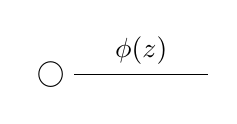
\begin{tikzpicture}
        \begin{feynman}
          % 顶点
          \vertex (a) at (0,0) {$\bigcirc $};
          \vertex [right=2cm of a] (b);
          
          % 粒子线
          \diagram* {
            (a) -- [solid,edge label=$\phi(z)$] (b)
          };
        \end{feynman}
    \end{tikzpicture}
\end{minipage}
\hfill
\begin{minipage}{0.5\textwidth}
    这是最简单的相互作用哈密顿量 $\hat{H}_I(z)$,它包含一个标量场 $\phi(z)$ 和一个源场 $J(z)$,
    \begin{equation*}
        \hat{H}_I(z) = J(z)\phi(z)
    \end{equation*}
\end{minipage}
\end{table}

\begin{table}[hbpt]
    \begin{minipage}{0.5\textwidth}
        \centering
        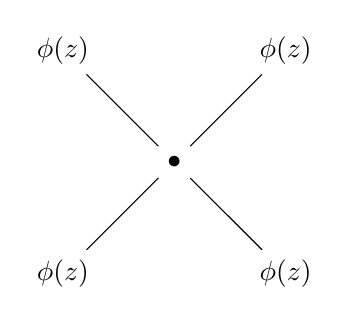
\begin{tikzpicture}
            \begin{feynman}
                \vertex (a) {$\bullet$};
                \vertex [above right=2cm of a] (b){$\phi(z)$};
                \vertex [below right=2cm of a] (c){$\phi(z)$};
                \vertex [above left=2cm of a] (d){$\phi(z)$};
                \vertex [below left=2cm of a] (e){$\phi(z)$};

                \diagram* {
                    (a) -- [solid] (b),
                    (a) -- [solid] (c),
                    (a) -- [solid] (d),
                    (a) -- [solid] (e)
                };
            \end{feynman}
        \end{tikzpicture}
    \end{minipage}
    \hfill
    \begin{minipage}{0.5\textwidth}
        这是最简单的自相互作用哈密顿量 $\hat{H}_I(z)$,我们一般将其称之为 $\phi^4$ 理论,其相互作用部分的哈密顿量为
        \begin{equation*}
            \hat{H}_I(z) = \frac{\lambda}{4!}\phi^4(z)
        \end{equation*}
    \end{minipage}
\end{table}

\begin{table}[hbpt]
    \begin{minipage}{0.5\textwidth}
        \centering
        \begin{tikzpicture}
            \begin{feynman}
                \vertex (a) ;
                \vertex [right=2cm of a] (b){$\phi(z)$};
                \vertex [above left=2cm of a] (c){$\psi^\dagger(z)$};
                \vertex [below left=2cm of a] (d){$\psi(z)$};
                \diagram* {
                    (a) -- [solid] (b),
                    (c) -- [anti fermion] (a),
                    (d) -- [fermion] (a)
                };
            \end{feynman}
        \end{tikzpicture}
    \end{minipage}
    \hfill
    \begin{minipage}{0.5\textwidth}
        这种相互作用是由 YuKawa 所提出的,其相互作用部分的哈密顿量 $\hat{H}_I(z)$为
        \begin{equation*}
            \hat{H}_I(z) = g \psi^\dagger(z)\psi(z)\phi(z)
        \end{equation*}
    \end{minipage}
\end{table}

\begin{table}[hbpt]
    \begin{minipage}{0.5\textwidth}
        \centering
        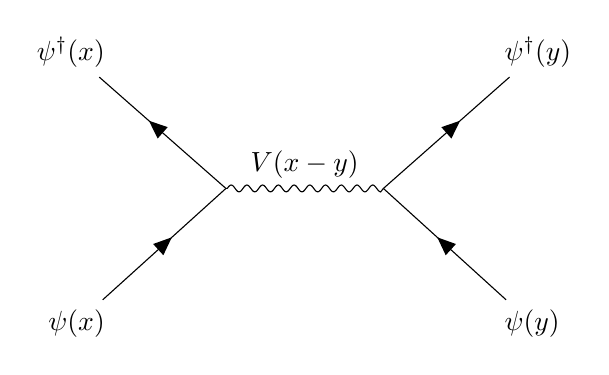
\begin{tikzpicture}
            \begin{feynman}
                \vertex (a) ;
                \vertex [right=2cm of a] (b);
                \vertex [above left=2cm of a] (c){$\psi^\dagger(x)$};
                \vertex [below left=2cm of a] (d){$\psi(x)$};
                \vertex [above right=2cm of b] (e){$\psi^\dagger(y)$};
                \vertex [below right=2cm of b] (f){$\psi(y)$};
                \diagram* {
                    (a) -- [boson,edge label=$V(x - y)$] (b),
                    (c) -- [anti fermion] (a),
                    (d) -- [fermion] (a),
                    (e) -- [anti fermion] (b),
                    (f) -- [fermion] (b)
                };
            \end{feynman}
        \end{tikzpicture}
    \end{minipage}
    \hfill
    \begin{minipage}{0.5\textwidth}
        最后一个例子是一种非常有用的非相对论的相互作用,其可以用来描述库伦相互作用,其相互作用部分的哈密顿量 $\hat{H}_I(z)$为
        \begin{equation*}
            \hat{H}_I(z) = \frac{1}{2}\psi^\dagger(x)\psi^\dagger(y)V(x - y)\delta(x^0 - y^0)\psi(y)\psi(x)
        \end{equation*}
    \end{minipage}
\end{table}

在介绍完一些相互作用以及图形上的表示之后,我们将会以 $\phi^4$ 相互作用作为例子来展开 $T[\hat{\phi}(x_1)\hat{\phi}(x_2)\hat{\phi}(x_3)\hat{\phi}(x_4)]$ 的真空期望值,首先,给出该相互作用的拉格朗日量
\begin{equation}
    \mathcal{L} = \frac{1}{2}\left[\partial_\mu \phi(x)\right]^2 - \frac{1}{2}m^2\phi^2(x) - \frac{\lambda}{4!}\phi^4(x)
\end{equation}

该拉格朗日量其前面一部分为自由 Klein-Gordon 场的拉格朗日量,我们可以将这部分通过正则量子化的方法得到系统的哈密顿量
\begin{equation}
    \hat{\mathcal{H}}_0 = \frac{1}{2}\left[\left(\frac{\partial \hat{\phi}}{\partial t}\right) + \left(\nabla\hat{\phi}\right)^2 + m^2\hat{\phi}^2\right] 
\end{equation}

而相互作用部分的哈密顿量则为
\begin{equation}
    \hat{\mathcal{H}}_I = \frac{\lambda}{4!}\phi^4(x)
\end{equation}

接下来,给出一个具体的过程来展开一下这个过程的 $\hat{S}$ 矩阵
\begin{example}
    考虑一个过程,其入态为一个处于 $p$ 的动量本征态的粒子,而其出态为一个处于 $q$ 的动量本征态的粒子,接下来计算一下这个过程的振幅
    \begin{solution}
        \begin{enumerate}
            \item[Step 1] 计算一下振幅 $\mathcal{A}$
            \begin{equation}
                \mathcal{A} = ^{out}\braket{q}{p}^{in} = \bra{q}\hat{S}\ket{p} = (2\pi)^3 \left(2E_{\vec{q}}\right)^{\frac{1}{2}} \left(2E_{\vec{p}}\right)^{\frac{1}{2}}\bra{0}\hat{a}_{\vec{q}}\hat{S}\hat{a}_{\vec{p}}^\dagger\ket{0}
            \end{equation}

            其中,我们的$\displaystyle \ket{p} = (2\pi)^\frac{3}{2} \left(2E_{\vec{q}}\right)^{\frac{1}{2}}\hat{a}_{\vec{p}}^\dagger\ket{0}$
            \item[Step 2] 将 $\hat{S}$ 从 Dyson's 表示进行展开,从而得到
            \begin{equation}
                \hat{S} = T\left[1 - \frac{i\lambda}{4!}\int d^4z \hat{\phi}^4(z) + \frac{\left(-i\right)^2}{2!}\left(\frac{\lambda}{4!}\right)^2 \int d^4 x d^4 y \hat{\phi}^4(x)\hat{\phi}^4(y) + \cdots\right]
            \end{equation}
            \item[Step 3] 将我们展开之后的 $\hat{S}$ 代入到 $\mathcal{A}$ 当中
            \begin{eqnarray*}
                \mathcal{A} &=& \bra{q}\hat{S}\ket{p} \\
                &=& (2\pi)^3 \left(2E_{\vec{q}}\right)^{\frac{1}{2}} \left(2E_{\vec{p}}\right)^{\frac{1}{2}} T\left[\bra{0}\hat{a}_{\vec{q}}\hat{a}_{\vec{p}}^\dagger\ket{0} + \int d^4z \left(\frac{-i\lambda}{4!}\right)\bra{0}\hat{a}_{\vec{q}}\hat{\phi}^4(z)\hat{a}_{\vec{p}}^\dagger\ket{0}\right. \\
                && \left. + \int d^4x d^4y \left(\frac{-i\lambda}{4!}\right)\bra{0}\hat{a}_{\vec{q}}\hat{\phi}^4(x)\hat{\phi}^4(y)\hat{a}_{\vec{p}}^\dagger\ket{0} + \cdots\right]
            \end{eqnarray*}

            于是,我们可以很自然的将振幅变成每一阶振幅的总和,即
            \begin{equation}
                \mathcal{A} = \mathcal{A}^{(0)} + \mathcal{A}^{(1)} + \mathcal{A}^{(2)} + \mathcal{A}^{(3)} + \cdots
            \end{equation}
            \item[Step 4] 得到了展开后的振幅之后,我们可以看出,真空期望值我们完全可以使用上一节得到的 Wick's Theorm 来展开,接下来开始
            \begin{itemize}
                \item 计算领头阶的真空期望值,这很容易
                \begin{equation*}
                    \mathcal{A}^{(0)} \propto T\left[\bra{0}\hat{a}_{\vec{q}}\hat{a}_{\vec{p}}^\dagger\ket{0}\right] = \wick{\c1 a_{\vec{q}} \c1 a_{\vec{p}}} = \delta^{(3)}(\vec{q} - \vec{p})
                \end{equation*}
                \item 计算一下较为复杂的一阶振幅当中的真空期望值,通过 wick constraction 我们可以得到
                \begin{eqnarray*}
                    \mathcal{A}^{(1)} &\propto& \int d^4z \left(\frac{-i\lambda}{4!}\right)\bra{0}T[\hat{a}_{\vec{q}}\hat{\phi}^4(z)\hat{a}_{\vec{p}}^\dagger]\ket{0} \\
                    &=& \int d^4z \left(\frac{-i\lambda}{4!}\right)\left[3 \bra{0} \hat{a}_{\vec{q}}\hat{a}_{\vec{p}}^\dagger\ket{0}\bra{0} \hat{\phi}(x)\hat{\phi}(x) \ket{0}\bra{0} \hat{\phi}(x)\hat{\phi}(x) \ket{0} + 12 \bra{0} \hat{a}_{\vec{q}}\hat{\phi}\ket{0}\bra{0} \hat{\phi}\hat{\phi}\ket{0}\bra{0} \hat{\phi}\hat{a}_{\vec{p}}^\dagger\ket{0} \right]
                \end{eqnarray*}

                这很复杂(至少对我来说),我们需要分别计算一下这里面出现的几个真空期望值,借用一下之前的结论(我们考虑的是一个自由标量场的 $\phi^4$ 理论),其场算符在 $\ket{p}$ 的动量本征态下的形式为
                \begin{equation}
                    \hat{\phi}(z) = \int \frac{d^3 \vec{p}}{\left(2\pi\right)^{\frac{3}{2}}} \frac{1}{\left(2 E_{\vec{p}}\right)^{\frac{1}{2}}}\left(\hat{a}_{\vec{p}}e^{-ip \cdot z} + \hat{a}_{\vec{p}}^\dagger e^{ip \cdot z}\right)
                \end{equation}

                根据该场算符的形式,我们可以计算得到
                \begin{eqnarray*}
                    \bra{0} \hat{\phi}\hat{\phi} \ket{0} &=& \Delta(z - z)\\
                    &=& \int \frac{d^4 k}{(2\pi)^4} \frac{e^{-ik(z - z)}}{k^2 - m^2 + i\epsilon}\\
                    \bra{0} \hat{a}_{\vec{q}}\hat{\phi} \ket{0} &=& \int d^3 \vec{q} d^3 \vec{p} \braket{\vec{q}}{\vec{p}}e^{i p \cdot z} \\
                    &=& \int d^3 \vec{q} e^{iq\cdot z} \\
                    \bra{0} \hat{\phi}\hat{a}_{\vec{p}}^\dagger \ket{0} &=& 
                \end{eqnarray*}
                \item 
            \end{itemize}
            \item[Step 5] 
        \end{enumerate}
    \end{solution}
\end{example}








\section{\protect\hyperlink{:}{散射振幅与其计算}}
\addtocontents{toc}{\protect\hypertarget{:}{}}







\chapter{\protect\hyperlink{:}{附录}}
\addtocontents{toc}{\protect\hypertarget{:}{}}


\section{\protect\hyperlink{:}{微分形式}}
\addtocontents{toc}{\protect\hypertarget{:}{}}

微分形式是一个数学里的一种方法,利用这种方法,在力学当中将会有很大的便利。

首先,这是一个在研究多元函数微积分的时候所引入的,那么我们就从此处开始。假设我们有一个二元函数 $f(x,y)$ ,我们现在研究一下他的二重积分

\begin{equation}\label{eq:double_integral}
    I = \iint_D f(x,y) dx dy
\end{equation}

在大多数情况下,我们可以直接求解这个二重积分,但是有的时候,我们需要对这个二重积分的变量进行代换以此来简化计算
\begin{equation}
    \begin{cases}
        x = x(u,v) \\
        y = y(u,v)
    \end{cases}
\end{equation}

在此变量代换下,我们的积分将变为
\begin{equation}
    I = \iint f(x,y) \left| \frac{\partial(x,y)}{\partial(u,v)} \right| du dv
\end{equation}

其中 $\displaystyle \left| \frac{\partial(x,y)}{\partial(u,v)} \right| = \frac{\partial x}{\partial u}\frac{\partial y}{\partial v} - \frac{\partial x}{\partial v}\frac{\partial y}{\partial u}$ 为坐标变换的雅可比行列式。这就告诉我们,坐标变换之后,我们还需要给被积函数乘上一个雅可比行列式,但是除此以外,我们还可以使用外代数的一种代数乘法来进行代替。

首先,我们可以将之前的二元积分 $\ref{eq:double_integral}$ 的积分微元 $dxdy$ 重写为 $dx \wedge dy$ ,我们将其称之为 \textbf{外积} ,这种乘法满足关系
\begin{equation}
    dx \wedge dy = -dy \wedge dx
\end{equation}

这也就是说,外积运算不能够对易,但是是反对易的,因此我们也会得到这样的关系
\begin{equation}
    dx \wedge dx = - dx \wedge dx = 0,\qquad dy \wedge dy = - dy \wedge dy = 0
\end{equation}

有了这个外代数,我们来计算一下上面的二重积分 $\ref{eq:double_integral}$ 的积分微元在坐标变换下的表现
\begin{eqnarray}
    dx \wedge dy &=& \left(\frac{\partial x}{\partial u} du + \frac{\partial y}{\partial v} dv\right) \wedge \left(\frac{\partial y}{\partial u} du + \frac{\partial y}{\partial v} dv\right) \nonumber \\
    &=& \frac{\partial x}{\partial u} \frac{\partial y}{\partial v} du \wedge dv + \frac{\partial y}{\partial u} \frac{\partial x}{\partial v} dv \wedge du \nonumber \\
    &=& \left(\frac{\partial x}{\partial u} \frac{\partial y}{\partial v} - \frac{\partial y}{\partial u} \frac{\partial x}{\partial v}\right) du \wedge dv \nonumber \\
    &=& \left| \frac{\partial(x,y)}{\partial(u,v)} \right| du \wedge dv
\end{eqnarray}

可以看到,利用外代数二元函数积分的坐标变换多出来的雅可比行列式自动就出现了那么同理,对于一个 $n$ 元函数积分,我们可以将其积分微元写成
\begin{equation}
    dx^1 \wedge dx^2 \wedge \cdots \wedge dx^n
\end{equation}

他们之间满足
\begin{equation}
    dx^i \wedge dx^j = -dx^j \wedge dx^i,\qquad dx^i \wedge dx^i = 0
\end{equation}

接下来,我们将被积函数 $f(x^1,x^2,\cdots,x^n)$ 和 积分微元 $dx^1 \wedge dx^2 \wedge \cdots \wedge dx^n$ 乘在一起称为 $n$ 重微分形式,简称 $n$ 形式,记作 $\omega$
\begin{equation}
    \omega = f(x^1,x^2,\cdots,x^n) dx^1 \wedge dx^2 \wedge \cdots \wedge dx^n
\end{equation} 

而 $n$ 重积分则被记为
\begin{equation}
    I = \int_D \omega
\end{equation}












\section{\protect\hyperlink{:}{张量代数}}
\addtocontents{toc}{\protect\hypertarget{:}{}}





\section{\protect\hyperlink{:}{Numerator Algebra}}
\addtocontents{toc}{\protect\hypertarget{:}{}}
Pauli matrix:
\begin{equation}
    \sigma^1 = 
    \begin{pmatrix}
        0 & 1 \\
        1 & 0
    \end{pmatrix},
    \sigma^2 =
    \begin{pmatrix}
        0 & -i \\
        i & 0
    \end{pmatrix},
    \sigma^3 =
    \begin{pmatrix}
        1 & 0 \\
        0 & -1
    \end{pmatrix}
\end{equation}

将其整合成一个四元组,得到我们的类似于四矢量形式的泡利矩阵:
\begin{equation}
    \sigma^\mu = \left(1,\vec{\sigma}\right),\qquad \bar{\sigma}^\mu = \left(1,-\vec{\sigma}\right)
\end{equation}

这两个新的 Pauli matirx 代表一个由单位矩阵和三个标准的泡利矩阵组成的四元组 $2 \times 2$ 矩阵,它在相对论量子力学中扮演着重要的角色,用于将三维的旋量和矢量推广到满足洛伦兹不变性的四维形式。

于是我们有 Dirac Matrix:
\begin{equation}
    \gamma^\mu = 
    \begin{pmatrix}
        0 & \sigma^\mu \\
        \bar{\sigma}^\mu & 0
    \end{pmatrix},
    \qquad \gamma^5 = \gamma^0\gamma^1\gamma^2\gamma^3 = 
    \begin{pmatrix}
        -1 & 0 \\
        0 & 1
    \end{pmatrix}
\end{equation}

其所遵循的反对易关系
\begin{equation}
    \left\{\gamma^\mu,\gamma^\nu\right\} = 2 g^{\mu\nu}
\end{equation}


Simplify the $\gamma$ matrix\cite{2}:

\begin{eqnarray*}
    \gamma^\mu \gamma_\mu &=& 4 \\
    \gamma^\mu \gamma^\nu \gamma_\mu &=& -2 \gamma^\nu \\
    \gamma^\mu \gamma^\nu \gamma^\rho \gamma_\mu &=& 4 g^{\nu\rho} \\
    \gamma^\mu \gamma^\nu \gamma^\rho \gamma^\sigma \gamma_\mu &=& -2 \gamma^\sigma \gamma^\rho \gamma^\nu
\end{eqnarray*}

Trace of $\gamma$ matrix:
\begin{eqnarray*}
    \tr(\mathbf{1}) &=& 4\\
    \tr( any\ odd\ \#\  of\ \gamma) &=& 0 \\
    \tr(\gamma^\mu\gamma^\nu) &=& 4g^{\mu\nu} \\
    \tr(\gamma^\mu\gamma^\nu\gamma^\rho\gamma^\sigma) &=& 4\left(g^{\mu\nu}g^{\rho\sigma} - g^{\mu\rho}g^{\nu\sigma} + g^{\mu\sigma}g^{\nu\rho}\right) \\
    \tr(\gamma^5) &=& 0 \\
    \tr(\gamma^\mu\gamma^\nu\gamma^5) &=& 0 \\
    \tr(\gamma^\mu\gamma^\nu\gamma^\rho\gamma^\sigma\gamma^5) &=& -4i\epsilon^{\mu\nu\rho\sigma} 
\end{eqnarray*}





\section{\protect\hyperlink{:}{Polarization of External Particles}}
\addtocontents{toc}{\protect\hypertarget{:}{}}





\section{\protect\hyperlink{:}{Feynman Rules}}
\addtocontents{toc}{\protect\hypertarget{:}{}}






\end{document}